\documentclass[twoside]{book}

% Packages required by doxygen
\usepackage{fixltx2e}
\usepackage{calc}
\usepackage{doxygen}
\usepackage[export]{adjustbox} % also loads graphicx
\usepackage{graphicx}
\usepackage[utf8]{inputenc}
\usepackage{makeidx}
\usepackage{multicol}
\usepackage{multirow}
\PassOptionsToPackage{warn}{textcomp}
\usepackage{textcomp}
\usepackage[nointegrals]{wasysym}
\usepackage[table]{xcolor}

% Font selection
\usepackage[T1]{fontenc}
\usepackage[scaled=.90]{helvet}
\usepackage{courier}
\usepackage{amssymb}
\usepackage{sectsty}
\renewcommand{\familydefault}{\sfdefault}
\allsectionsfont{%
  \fontseries{bc}\selectfont%
  \color{darkgray}%
}
\renewcommand{\DoxyLabelFont}{%
  \fontseries{bc}\selectfont%
  \color{darkgray}%
}
\newcommand{\+}{\discretionary{\mbox{\scriptsize$\hookleftarrow$}}{}{}}

% Page & text layout
\usepackage{geometry}
\geometry{%
  a4paper,%
  top=2.5cm,%
  bottom=2.5cm,%
  left=2.5cm,%
  right=2.5cm%
}
\tolerance=750
\hfuzz=15pt
\hbadness=750
\setlength{\emergencystretch}{15pt}
\setlength{\parindent}{0cm}
\setlength{\parskip}{3ex plus 2ex minus 2ex}
\makeatletter
\renewcommand{\paragraph}{%
  \@startsection{paragraph}{4}{0ex}{-1.0ex}{1.0ex}{%
    \normalfont\normalsize\bfseries\SS@parafont%
  }%
}
\renewcommand{\subparagraph}{%
  \@startsection{subparagraph}{5}{0ex}{-1.0ex}{1.0ex}{%
    \normalfont\normalsize\bfseries\SS@subparafont%
  }%
}
\makeatother

% Headers & footers
\usepackage{fancyhdr}
\pagestyle{fancyplain}
\fancyhead[LE]{\fancyplain{}{\bfseries\thepage}}
\fancyhead[CE]{\fancyplain{}{}}
\fancyhead[RE]{\fancyplain{}{\bfseries\leftmark}}
\fancyhead[LO]{\fancyplain{}{\bfseries\rightmark}}
\fancyhead[CO]{\fancyplain{}{}}
\fancyhead[RO]{\fancyplain{}{\bfseries\thepage}}
\fancyfoot[LE]{\fancyplain{}{}}
\fancyfoot[CE]{\fancyplain{}{}}
\fancyfoot[RE]{\fancyplain{}{\bfseries\scriptsize Generated by Doxygen }}
\fancyfoot[LO]{\fancyplain{}{\bfseries\scriptsize Generated by Doxygen }}
\fancyfoot[CO]{\fancyplain{}{}}
\fancyfoot[RO]{\fancyplain{}{}}
\renewcommand{\footrulewidth}{0.4pt}
\renewcommand{\chaptermark}[1]{%
  \markboth{#1}{}%
}
\renewcommand{\sectionmark}[1]{%
  \markright{\thesection\ #1}%
}

% Indices & bibliography
\usepackage{natbib}
\usepackage[titles]{tocloft}
\setcounter{tocdepth}{3}
\setcounter{secnumdepth}{5}
\makeindex

% Hyperlinks (required, but should be loaded last)
\usepackage{ifpdf}
\ifpdf
  \usepackage[pdftex,pagebackref=true]{hyperref}
\else
  \usepackage[ps2pdf,pagebackref=true]{hyperref}
\fi
\hypersetup{%
  colorlinks=true,%
  linkcolor=blue,%
  citecolor=blue,%
  unicode%
}

% Custom commands
\newcommand{\clearemptydoublepage}{%
  \newpage{\pagestyle{empty}\cleardoublepage}%
}

\usepackage{caption}
\captionsetup{labelsep=space,justification=centering,font={bf},singlelinecheck=off,skip=4pt,position=top}

%===== C O N T E N T S =====

\begin{document}

% Titlepage & ToC
\hypersetup{pageanchor=false,
             bookmarksnumbered=true,
             pdfencoding=unicode
            }
\pagenumbering{alph}
\begin{titlepage}
\vspace*{7cm}
\begin{center}%
{\Large My Project }\\
\vspace*{1cm}
{\large Generated by Doxygen 1.8.13}\\
\end{center}
\end{titlepage}
\clearemptydoublepage
\pagenumbering{roman}
\tableofcontents
\clearemptydoublepage
\pagenumbering{arabic}
\hypersetup{pageanchor=true}

%--- Begin generated contents ---
\chapter{Examen\+Embebidos2}
\label{md__home_jonacb_stm32_ExamenEmbebidos2_README}
\Hypertarget{md__home_jonacb_stm32_ExamenEmbebidos2_README}
\input{md__home_jonacb_stm32_ExamenEmbebidos2_README}
\chapter{Class Index}
\doxysection{Data Structures}
Here are the data structures with brief descriptions\+:\begin{DoxyCompactList}
\item\contentsline{section}{\mbox{\hyperlink{structs__internal}{s\+\_\+internal}} }{\pageref{structs__internal}}{}
\item\contentsline{section}{\mbox{\hyperlink{structs__mini__args}{s\+\_\+mini\+\_\+args}} }{\pageref{structs__mini__args}}{}
\item\contentsline{section}{\mbox{\hyperlink{structs__mini__sprintf}{s\+\_\+mini\+\_\+sprintf}} }{\pageref{structs__mini__sprintf}}{}
\end{DoxyCompactList}

\chapter{File Index}
\doxysection{File List}
Here is a list of all documented files with brief descriptions\+:\begin{DoxyCompactList}
\item\contentsline{section}{Git\+Hub/\+Sistemas\+Embebidos\+Tec\+G\+D\+A/\+Abstraction\+\_\+and\+\_\+documentation/dimmer/\mbox{\hyperlink{dimmer_8c}{dimmer.\+c}} }{\pageref{dimmer_8c}}{}
\item\contentsline{section}{Git\+Hub/\+Sistemas\+Embebidos\+Tec\+G\+D\+A/\+Abstraction\+\_\+and\+\_\+documentation/dimmer/{\bfseries dimmer.\+h} }{\pageref{dimmer_8h}}{}
\item\contentsline{section}{Git\+Hub/\+Sistemas\+Embebidos\+Tec\+G\+D\+A/\+Abstraction\+\_\+and\+\_\+documentation/dimmer/{\bfseries dimmer\+\_\+params.\+h} }{\pageref{dimmer__params_8h}}{}
\item\contentsline{section}{Git\+Hub/\+Sistemas\+Embebidos\+Tec\+G\+D\+A/\+Abstraction\+\_\+and\+\_\+documentation/i2c\+\_\+adc/\mbox{\hyperlink{i2c__adc_8c}{i2c\+\_\+adc.\+c}} }{\pageref{i2c__adc_8c}}{}
\item\contentsline{section}{Git\+Hub/\+Sistemas\+Embebidos\+Tec\+G\+D\+A/\+Abstraction\+\_\+and\+\_\+documentation/i2c\+\_\+adc/{\bfseries i2c\+\_\+adc.\+h} }{\pageref{i2c__adc_8h}}{}
\item\contentsline{section}{Git\+Hub/\+Sistemas\+Embebidos\+Tec\+G\+D\+A/\+Abstraction\+\_\+and\+\_\+documentation/miniprintf/{\bfseries miniprintf.\+h} }{\pageref{miniprintf_8h}}{}
\item\contentsline{section}{Git\+Hub/\+Sistemas\+Embebidos\+Tec\+G\+D\+A/\+Abstraction\+\_\+and\+\_\+documentation/system\+\_\+common/\mbox{\hyperlink{system__common_8c}{system\+\_\+common.\+c}} }{\pageref{system__common_8c}}{}
\item\contentsline{section}{Git\+Hub/\+Sistemas\+Embebidos\+Tec\+G\+D\+A/\+Abstraction\+\_\+and\+\_\+documentation/system\+\_\+common/{\bfseries system\+\_\+common.\+h} }{\pageref{system__common_8h}}{}
\item\contentsline{section}{Git\+Hub/\+Sistemas\+Embebidos\+Tec\+G\+D\+A/\+Abstraction\+\_\+and\+\_\+documentation/temp\+\_\+sensor/\mbox{\hyperlink{temp__sensor_8c}{temp\+\_\+sensor.\+c}} }{\pageref{temp__sensor_8c}}{}
\item\contentsline{section}{Git\+Hub/\+Sistemas\+Embebidos\+Tec\+G\+D\+A/\+Abstraction\+\_\+and\+\_\+documentation/temp\+\_\+sensor/{\bfseries temp\+\_\+sensor.\+h} }{\pageref{temp__sensor_8h}}{}
\item\contentsline{section}{Git\+Hub/\+Sistemas\+Embebidos\+Tec\+G\+D\+A/\+Abstraction\+\_\+and\+\_\+documentation/temp\+\_\+sensor/{\bfseries temp\+\_\+sensor\+\_\+params.\+h} }{\pageref{temp__sensor__params_8h}}{}
\item\contentsline{section}{Git\+Hub/\+Sistemas\+Embebidos\+Tec\+G\+D\+A/\+Abstraction\+\_\+and\+\_\+documentation/uc\+\_\+adc/\mbox{\hyperlink{uc__adc_8c}{uc\+\_\+adc.\+c}} }{\pageref{uc__adc_8c}}{}
\item\contentsline{section}{Git\+Hub/\+Sistemas\+Embebidos\+Tec\+G\+D\+A/\+Abstraction\+\_\+and\+\_\+documentation/uc\+\_\+adc/{\bfseries uc\+\_\+adc.\+h} }{\pageref{uc__adc_8h}}{}
\item\contentsline{section}{Git\+Hub/\+Sistemas\+Embebidos\+Tec\+G\+D\+A/\+Abstraction\+\_\+and\+\_\+documentation/uc\+\_\+i2c/\mbox{\hyperlink{uc__i2c_8c}{uc\+\_\+i2c.\+c}} }{\pageref{uc__i2c_8c}}{}
\item\contentsline{section}{Git\+Hub/\+Sistemas\+Embebidos\+Tec\+G\+D\+A/\+Abstraction\+\_\+and\+\_\+documentation/uc\+\_\+i2c/{\bfseries uc\+\_\+i2c.\+h} }{\pageref{uc__i2c_8h}}{}
\item\contentsline{section}{Git\+Hub/\+Sistemas\+Embebidos\+Tec\+G\+D\+A/\+Abstraction\+\_\+and\+\_\+documentation/uc\+\_\+interrupt/\mbox{\hyperlink{uc__interrupt_8c}{uc\+\_\+interrupt.\+c}} }{\pageref{uc__interrupt_8c}}{}
\item\contentsline{section}{Git\+Hub/\+Sistemas\+Embebidos\+Tec\+G\+D\+A/\+Abstraction\+\_\+and\+\_\+documentation/uc\+\_\+interrupt/{\bfseries uc\+\_\+interrupt.\+h} }{\pageref{uc__interrupt_8h}}{}
\item\contentsline{section}{Git\+Hub/\+Sistemas\+Embebidos\+Tec\+G\+D\+A/\+Abstraction\+\_\+and\+\_\+documentation/uc\+\_\+timer/\mbox{\hyperlink{uc__timer_8c}{uc\+\_\+timer.\+c}} }{\pageref{uc__timer_8c}}{}
\item\contentsline{section}{Git\+Hub/\+Sistemas\+Embebidos\+Tec\+G\+D\+A/\+Abstraction\+\_\+and\+\_\+documentation/uc\+\_\+timer/{\bfseries uc\+\_\+timer.\+h} }{\pageref{uc__timer_8h}}{}
\item\contentsline{section}{Git\+Hub/\+Sistemas\+Embebidos\+Tec\+G\+D\+A/\+Abstraction\+\_\+and\+\_\+documentation/uc\+\_\+uart/\mbox{\hyperlink{uc__uart_8c}{uc\+\_\+uart.\+c}} }{\pageref{uc__uart_8c}}{}
\item\contentsline{section}{Git\+Hub/\+Sistemas\+Embebidos\+Tec\+G\+D\+A/\+Abstraction\+\_\+and\+\_\+documentation/uc\+\_\+uart/{\bfseries uc\+\_\+uart.\+h} }{\pageref{uc__uart_8h}}{}
\end{DoxyCompactList}

\chapter{Class Documentation}
\hypertarget{structs__internal}{}\section{s\+\_\+internal Struct Reference}
\label{structs__internal}\index{s\+\_\+internal@{s\+\_\+internal}}
\subsection*{Public Attributes}
\begin{DoxyCompactItemize}
\item 
void($\ast$ \hyperlink{structs__internal_a046caf8bd89d8e15e72d1343200347ec}{putc} )(char)
\item 
unsigned \hyperlink{structs__internal_aa5f781ae7e2d8c24589aa3baa43eaeec}{count}
\item 
unsigned \hyperlink{structs__internal_a8b552ee95b8f39562944aa3b19de3a85}{cooked}\+: 1
\end{DoxyCompactItemize}


\subsection{Detailed Description}
\hyperlink{structs__internal}{s\+\_\+internal} trackes the count of bytes output\+: 

\subsection{Member Data Documentation}
\mbox{\Hypertarget{structs__internal_a8b552ee95b8f39562944aa3b19de3a85}\label{structs__internal_a8b552ee95b8f39562944aa3b19de3a85}} 
\index{s\+\_\+internal@{s\+\_\+internal}!cooked@{cooked}}
\index{cooked@{cooked}!s\+\_\+internal@{s\+\_\+internal}}
\subsubsection{\texorpdfstring{cooked}{cooked}}
{\footnotesize\ttfamily unsigned s\+\_\+internal\+::cooked}

When true, \textquotesingle{}~\newline
\textquotesingle{} also emits \textquotesingle{}\textquotesingle{} \mbox{\Hypertarget{structs__internal_aa5f781ae7e2d8c24589aa3baa43eaeec}\label{structs__internal_aa5f781ae7e2d8c24589aa3baa43eaeec}} 
\index{s\+\_\+internal@{s\+\_\+internal}!count@{count}}
\index{count@{count}!s\+\_\+internal@{s\+\_\+internal}}
\subsubsection{\texorpdfstring{count}{count}}
{\footnotesize\ttfamily unsigned s\+\_\+internal\+::count}

Bytes output \mbox{\Hypertarget{structs__internal_a046caf8bd89d8e15e72d1343200347ec}\label{structs__internal_a046caf8bd89d8e15e72d1343200347ec}} 
\index{s\+\_\+internal@{s\+\_\+internal}!putc@{putc}}
\index{putc@{putc}!s\+\_\+internal@{s\+\_\+internal}}
\subsubsection{\texorpdfstring{putc}{putc}}
{\footnotesize\ttfamily void($\ast$ s\+\_\+internal\+::putc) (char)}

User\textquotesingle{}s \hyperlink{structs__internal_a046caf8bd89d8e15e72d1343200347ec}{putc()} routine to be used 

The documentation for this struct was generated from the following file\+:\begin{DoxyCompactItemize}
\item 
/home/jonacb/stm32/\+Examen\+Embebidos2/miniprintf/\hyperlink{miniprintf_8c}{miniprintf.\+c}\end{DoxyCompactItemize}

\hypertarget{structs__mini__args}{}\section{s\+\_\+mini\+\_\+args Struct Reference}
\label{structs__mini__args}\index{s\+\_\+mini\+\_\+args@{s\+\_\+mini\+\_\+args}}
\subsection*{Public Attributes}
\begin{DoxyCompactItemize}
\item 
\mbox{\Hypertarget{structs__mini__args_a150c5c7a07d3aa0301fae09b17d3e43f}\label{structs__mini__args_a150c5c7a07d3aa0301fae09b17d3e43f}} 
void($\ast$ \hyperlink{structs__mini__args_a150c5c7a07d3aa0301fae09b17d3e43f}{putc} )(char, void $\ast$)
\begin{DoxyCompactList}\small\item\em The \hyperlink{structs__mini__args_a150c5c7a07d3aa0301fae09b17d3e43f}{putc()} function to invoke. \end{DoxyCompactList}\item 
\mbox{\Hypertarget{structs__mini__args_ae4547bc8c8a470df0e6d60b02d15ed37}\label{structs__mini__args_ae4547bc8c8a470df0e6d60b02d15ed37}} 
void $\ast$ \hyperlink{structs__mini__args_ae4547bc8c8a470df0e6d60b02d15ed37}{argp}
\begin{DoxyCompactList}\small\item\em Associated data struct. \end{DoxyCompactList}\end{DoxyCompactItemize}


\subsection{Detailed Description}
Minimal printf() facility for M\+C\+Us Warren W. Gay V\+E3\+W\+WG, Sun Feb 12 2017

This work is placed in the public domain. No warranty, or guarantee is expressed or implied. When uou use this source code, you do so with full responsibility and at your own risk.

Internal structure for I/O 

The documentation for this struct was generated from the following file\+:\begin{DoxyCompactItemize}
\item 
/home/jonacb/stm32/\+Examen\+Embebidos2/miniprintf/\hyperlink{miniprintf_8c}{miniprintf.\+c}\end{DoxyCompactItemize}

\hypertarget{structs__mini__sprintf}{}\doxysection{s\+\_\+mini\+\_\+sprintf Struct Reference}
\label{structs__mini__sprintf}\index{s\_mini\_sprintf@{s\_mini\_sprintf}}
\doxysubsection*{Data Fields}
\begin{DoxyCompactItemize}
\item 
\mbox{\Hypertarget{structs__mini__sprintf_a1fe855c208bc17a51a4d34fefdb2d5b1}\label{structs__mini__sprintf_a1fe855c208bc17a51a4d34fefdb2d5b1}} 
char $\ast$ {\bfseries buf}
\item 
\mbox{\Hypertarget{structs__mini__sprintf_afecf7a1c0875af08584fc97840095978}\label{structs__mini__sprintf_afecf7a1c0875af08584fc97840095978}} 
unsigned {\bfseries maxbuf}
\item 
\mbox{\Hypertarget{structs__mini__sprintf_a935adc2e417a61d7eb6f04efb18ba031}\label{structs__mini__sprintf_a935adc2e417a61d7eb6f04efb18ba031}} 
char $\ast$ {\bfseries ptr}
\end{DoxyCompactItemize}


The documentation for this struct was generated from the following file\+:\begin{DoxyCompactItemize}
\item 
Git\+Hub/\+Sistemas\+Embebidos\+Tec\+G\+D\+A/\+Abstraction\+\_\+and\+\_\+documentation/miniprintf/miniprintf.\+c\end{DoxyCompactItemize}

\chapter{File Documentation}
\hypertarget{buttons_8c}{}\section{/home/jonacb/stm32/\+Examen\+Embebidos2/buttons/buttons.c File Reference}
\label{buttons_8c}\index{/home/jonacb/stm32/\+Examen\+Embebidos2/buttons/buttons.\+c@{/home/jonacb/stm32/\+Examen\+Embebidos2/buttons/buttons.\+c}}


Button function definitions.  


{\ttfamily \#include \char`\"{}buttons.\+h\char`\"{}}\newline
{\ttfamily \#include \char`\"{}../gpio/gpio.\+h\char`\"{}}\newline
Include dependency graph for buttons.\+c\+:\nopagebreak
\begin{figure}[H]
\begin{center}
\leavevmode
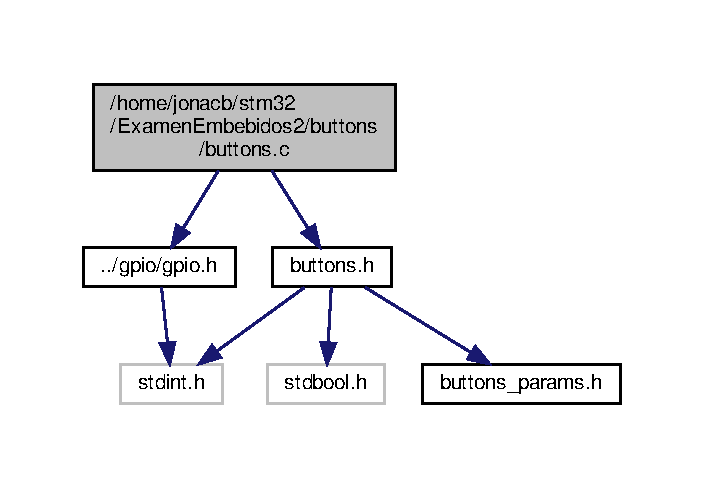
\includegraphics[width=338pt]{buttons_8c__incl}
\end{center}
\end{figure}
\subsection*{Functions}
\begin{DoxyCompactItemize}
\item 
void \hyperlink{buttons_8c_a58f9788bfb584a5b915ffff18d3bc410}{buttons\+\_\+setup} (void)
\begin{DoxyCompactList}\small\item\em Sets up the buttons needed for this project. \end{DoxyCompactList}\item 
bool \hyperlink{buttons_8c_a096706e90277a8acaccd45febdc3371c}{reset\+\_\+button\+\_\+pressed} (void)
\begin{DoxyCompactList}\small\item\em Returns whether the reset button is pressed. \end{DoxyCompactList}\item 
bool \hyperlink{buttons_8c_a1af30191280bf4afc129021651902ff7}{start\+\_\+button\+\_\+pressed} (void)
\begin{DoxyCompactList}\small\item\em Returns whether the start button is pressed. \end{DoxyCompactList}\item 
bool \hyperlink{buttons_8c_ae1caa49be6beb3becba7b993589aaf32}{stop\+\_\+button\+\_\+pressed} (void)
\begin{DoxyCompactList}\small\item\em Returns whether the stop button is pressed. \end{DoxyCompactList}\end{DoxyCompactItemize}


\subsection{Detailed Description}
Button function definitions. 



\subsection{Function Documentation}
\mbox{\Hypertarget{buttons_8c_a58f9788bfb584a5b915ffff18d3bc410}\label{buttons_8c_a58f9788bfb584a5b915ffff18d3bc410}} 
\index{buttons.\+c@{buttons.\+c}!buttons\+\_\+setup@{buttons\+\_\+setup}}
\index{buttons\+\_\+setup@{buttons\+\_\+setup}!buttons.\+c@{buttons.\+c}}
\subsubsection{\texorpdfstring{buttons\+\_\+setup()}{buttons\_setup()}}
{\footnotesize\ttfamily void buttons\+\_\+setup (\begin{DoxyParamCaption}\item[{void}]{ }\end{DoxyParamCaption})}



Sets up the buttons needed for this project. 

$<$stdint library. stdbool library. button\+\_\+params header file. \mbox{\Hypertarget{buttons_8c_a096706e90277a8acaccd45febdc3371c}\label{buttons_8c_a096706e90277a8acaccd45febdc3371c}} 
\index{buttons.\+c@{buttons.\+c}!reset\+\_\+button\+\_\+pressed@{reset\+\_\+button\+\_\+pressed}}
\index{reset\+\_\+button\+\_\+pressed@{reset\+\_\+button\+\_\+pressed}!buttons.\+c@{buttons.\+c}}
\subsubsection{\texorpdfstring{reset\+\_\+button\+\_\+pressed()}{reset\_button\_pressed()}}
{\footnotesize\ttfamily bool reset\+\_\+button\+\_\+pressed (\begin{DoxyParamCaption}\item[{void}]{ }\end{DoxyParamCaption})}



Returns whether the reset button is pressed. 

\begin{DoxyReturn}{Returns}
reset\+\_\+button\+\_\+status 
\end{DoxyReturn}
\mbox{\Hypertarget{buttons_8c_a1af30191280bf4afc129021651902ff7}\label{buttons_8c_a1af30191280bf4afc129021651902ff7}} 
\index{buttons.\+c@{buttons.\+c}!start\+\_\+button\+\_\+pressed@{start\+\_\+button\+\_\+pressed}}
\index{start\+\_\+button\+\_\+pressed@{start\+\_\+button\+\_\+pressed}!buttons.\+c@{buttons.\+c}}
\subsubsection{\texorpdfstring{start\+\_\+button\+\_\+pressed()}{start\_button\_pressed()}}
{\footnotesize\ttfamily bool start\+\_\+button\+\_\+pressed (\begin{DoxyParamCaption}\item[{void}]{ }\end{DoxyParamCaption})}



Returns whether the start button is pressed. 

\begin{DoxyReturn}{Returns}
start\+\_\+button\+\_\+status 
\end{DoxyReturn}
\mbox{\Hypertarget{buttons_8c_ae1caa49be6beb3becba7b993589aaf32}\label{buttons_8c_ae1caa49be6beb3becba7b993589aaf32}} 
\index{buttons.\+c@{buttons.\+c}!stop\+\_\+button\+\_\+pressed@{stop\+\_\+button\+\_\+pressed}}
\index{stop\+\_\+button\+\_\+pressed@{stop\+\_\+button\+\_\+pressed}!buttons.\+c@{buttons.\+c}}
\subsubsection{\texorpdfstring{stop\+\_\+button\+\_\+pressed()}{stop\_button\_pressed()}}
{\footnotesize\ttfamily bool stop\+\_\+button\+\_\+pressed (\begin{DoxyParamCaption}\item[{void}]{ }\end{DoxyParamCaption})}



Returns whether the stop button is pressed. 

\begin{DoxyReturn}{Returns}
stop\+\_\+button\+\_\+status 
\end{DoxyReturn}

\hypertarget{buttons_8h}{}\section{/home/jonacb/stm32/\+Examen\+Embebidos2/buttons/buttons.h File Reference}
\label{buttons_8h}\index{/home/jonacb/stm32/\+Examen\+Embebidos2/buttons/buttons.\+h@{/home/jonacb/stm32/\+Examen\+Embebidos2/buttons/buttons.\+h}}


Button header file.  


{\ttfamily \#include $<$stdint.\+h$>$}\newline
{\ttfamily \#include $<$stdbool.\+h$>$}\newline
{\ttfamily \#include \char`\"{}buttons\+\_\+params.\+h\char`\"{}}\newline
Include dependency graph for buttons.\+h\+:\nopagebreak
\begin{figure}[H]
\begin{center}
\leavevmode
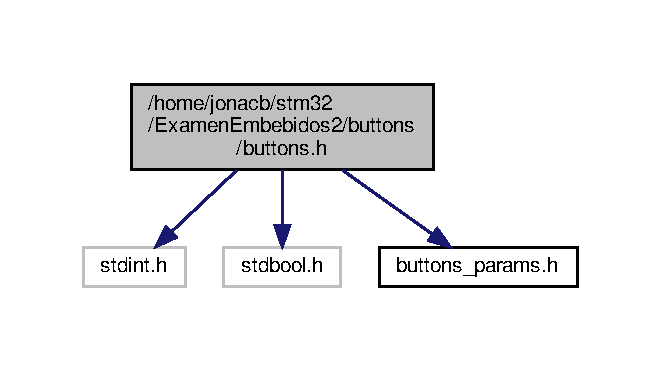
\includegraphics[width=317pt]{buttons_8h__incl}
\end{center}
\end{figure}
This graph shows which files directly or indirectly include this file\+:\nopagebreak
\begin{figure}[H]
\begin{center}
\leavevmode
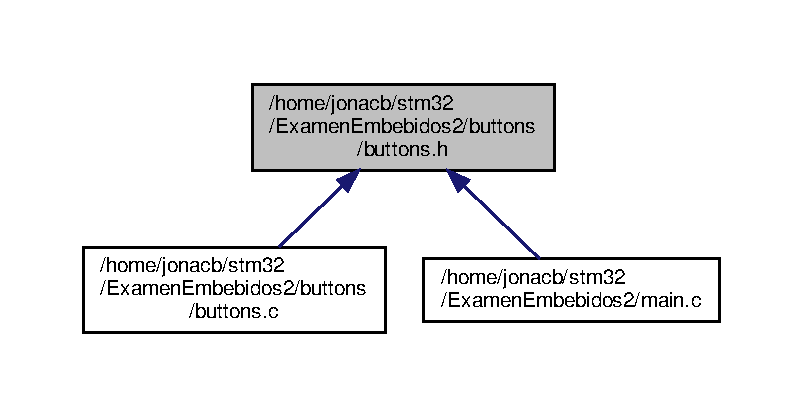
\includegraphics[width=350pt]{buttons_8h__dep__incl}
\end{center}
\end{figure}
\subsection*{Functions}
\begin{DoxyCompactItemize}
\item 
void \hyperlink{buttons_8h_a58f9788bfb584a5b915ffff18d3bc410}{buttons\+\_\+setup} (void)
\begin{DoxyCompactList}\small\item\em Sets up the buttons needed for this project. \end{DoxyCompactList}\item 
bool \hyperlink{buttons_8h_a096706e90277a8acaccd45febdc3371c}{reset\+\_\+button\+\_\+pressed} (void)
\begin{DoxyCompactList}\small\item\em Returns whether the reset button is pressed. \end{DoxyCompactList}\item 
bool \hyperlink{buttons_8h_a1af30191280bf4afc129021651902ff7}{start\+\_\+button\+\_\+pressed} (void)
\begin{DoxyCompactList}\small\item\em Returns whether the start button is pressed. \end{DoxyCompactList}\item 
bool \hyperlink{buttons_8h_ae1caa49be6beb3becba7b993589aaf32}{stop\+\_\+button\+\_\+pressed} (void)
\begin{DoxyCompactList}\small\item\em Returns whether the stop button is pressed. \end{DoxyCompactList}\end{DoxyCompactItemize}


\subsection{Detailed Description}
Button header file. 



\subsection{Function Documentation}
\mbox{\Hypertarget{buttons_8h_a58f9788bfb584a5b915ffff18d3bc410}\label{buttons_8h_a58f9788bfb584a5b915ffff18d3bc410}} 
\index{buttons.\+h@{buttons.\+h}!buttons\+\_\+setup@{buttons\+\_\+setup}}
\index{buttons\+\_\+setup@{buttons\+\_\+setup}!buttons.\+h@{buttons.\+h}}
\subsubsection{\texorpdfstring{buttons\+\_\+setup()}{buttons\_setup()}}
{\footnotesize\ttfamily void buttons\+\_\+setup (\begin{DoxyParamCaption}\item[{void}]{ }\end{DoxyParamCaption})}



Sets up the buttons needed for this project. 

$<$stdint library. stdbool library. button\+\_\+params header file. \mbox{\Hypertarget{buttons_8h_a096706e90277a8acaccd45febdc3371c}\label{buttons_8h_a096706e90277a8acaccd45febdc3371c}} 
\index{buttons.\+h@{buttons.\+h}!reset\+\_\+button\+\_\+pressed@{reset\+\_\+button\+\_\+pressed}}
\index{reset\+\_\+button\+\_\+pressed@{reset\+\_\+button\+\_\+pressed}!buttons.\+h@{buttons.\+h}}
\subsubsection{\texorpdfstring{reset\+\_\+button\+\_\+pressed()}{reset\_button\_pressed()}}
{\footnotesize\ttfamily bool reset\+\_\+button\+\_\+pressed (\begin{DoxyParamCaption}\item[{void}]{ }\end{DoxyParamCaption})}



Returns whether the reset button is pressed. 

\begin{DoxyReturn}{Returns}
reset\+\_\+button\+\_\+status 
\end{DoxyReturn}
\mbox{\Hypertarget{buttons_8h_a1af30191280bf4afc129021651902ff7}\label{buttons_8h_a1af30191280bf4afc129021651902ff7}} 
\index{buttons.\+h@{buttons.\+h}!start\+\_\+button\+\_\+pressed@{start\+\_\+button\+\_\+pressed}}
\index{start\+\_\+button\+\_\+pressed@{start\+\_\+button\+\_\+pressed}!buttons.\+h@{buttons.\+h}}
\subsubsection{\texorpdfstring{start\+\_\+button\+\_\+pressed()}{start\_button\_pressed()}}
{\footnotesize\ttfamily bool start\+\_\+button\+\_\+pressed (\begin{DoxyParamCaption}\item[{void}]{ }\end{DoxyParamCaption})}



Returns whether the start button is pressed. 

\begin{DoxyReturn}{Returns}
start\+\_\+button\+\_\+status 
\end{DoxyReturn}
\mbox{\Hypertarget{buttons_8h_ae1caa49be6beb3becba7b993589aaf32}\label{buttons_8h_ae1caa49be6beb3becba7b993589aaf32}} 
\index{buttons.\+h@{buttons.\+h}!stop\+\_\+button\+\_\+pressed@{stop\+\_\+button\+\_\+pressed}}
\index{stop\+\_\+button\+\_\+pressed@{stop\+\_\+button\+\_\+pressed}!buttons.\+h@{buttons.\+h}}
\subsubsection{\texorpdfstring{stop\+\_\+button\+\_\+pressed()}{stop\_button\_pressed()}}
{\footnotesize\ttfamily bool stop\+\_\+button\+\_\+pressed (\begin{DoxyParamCaption}\item[{void}]{ }\end{DoxyParamCaption})}



Returns whether the stop button is pressed. 

\begin{DoxyReturn}{Returns}
stop\+\_\+button\+\_\+status 
\end{DoxyReturn}

\hypertarget{buttons__params_8h}{}\section{/home/jonacb/stm32/\+Examen\+Embebidos2/buttons/buttons\+\_\+params.h File Reference}
\label{buttons__params_8h}\index{/home/jonacb/stm32/\+Examen\+Embebidos2/buttons/buttons\+\_\+params.\+h@{/home/jonacb/stm32/\+Examen\+Embebidos2/buttons/buttons\+\_\+params.\+h}}


Button parameters.  


This graph shows which files directly or indirectly include this file\+:\nopagebreak
\begin{figure}[H]
\begin{center}
\leavevmode
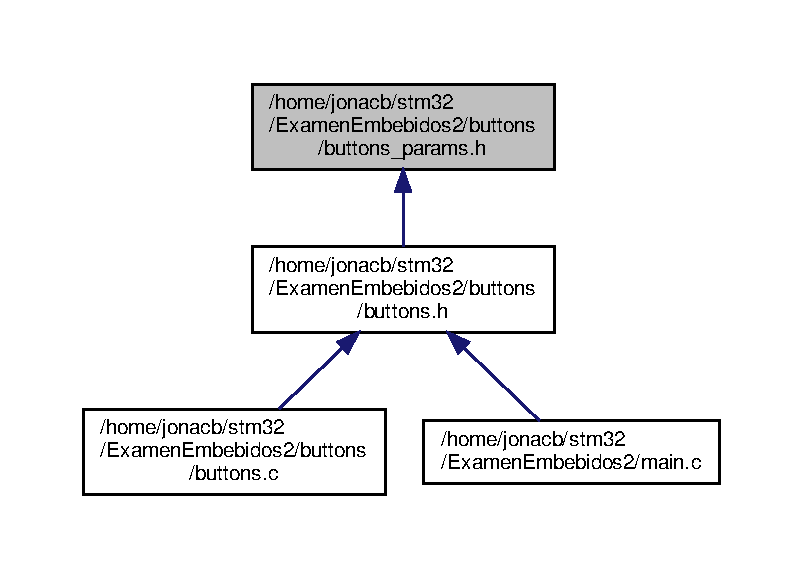
\includegraphics[width=350pt]{buttons__params_8h__dep__incl}
\end{center}
\end{figure}
\subsection*{Macros}
\begin{DoxyCompactItemize}
\item 
\mbox{\Hypertarget{buttons__params_8h_a5e26b1856a45389e5063f680b07c1cf8}\label{buttons__params_8h_a5e26b1856a45389e5063f680b07c1cf8}} 
\#define \hyperlink{buttons__params_8h_a5e26b1856a45389e5063f680b07c1cf8}{R\+E\+S\+E\+T\+\_\+\+B\+U\+T\+T\+O\+N\+\_\+\+P\+O\+RT}~1
\begin{DoxyCompactList}\small\item\em Reset button port. \end{DoxyCompactList}\item 
\mbox{\Hypertarget{buttons__params_8h_a56b64973bfd6514570671a2607122199}\label{buttons__params_8h_a56b64973bfd6514570671a2607122199}} 
\#define \hyperlink{buttons__params_8h_a56b64973bfd6514570671a2607122199}{R\+E\+S\+E\+T\+\_\+\+B\+U\+T\+T\+O\+N\+\_\+\+P\+IN}~1
\begin{DoxyCompactList}\small\item\em Reset button pin. \end{DoxyCompactList}\item 
\mbox{\Hypertarget{buttons__params_8h_a09e189758b3c4107df2b48ecd1466897}\label{buttons__params_8h_a09e189758b3c4107df2b48ecd1466897}} 
\#define \hyperlink{buttons__params_8h_a09e189758b3c4107df2b48ecd1466897}{S\+T\+A\+R\+T\+\_\+\+B\+U\+T\+T\+O\+N\+\_\+\+P\+O\+RT}~1
\begin{DoxyCompactList}\small\item\em Start button port. \end{DoxyCompactList}\item 
\mbox{\Hypertarget{buttons__params_8h_af727d34dc72e3f32bd32754111724a0b}\label{buttons__params_8h_af727d34dc72e3f32bd32754111724a0b}} 
\#define \hyperlink{buttons__params_8h_af727d34dc72e3f32bd32754111724a0b}{S\+T\+A\+R\+T\+\_\+\+B\+U\+T\+T\+O\+N\+\_\+\+P\+IN}~1
\begin{DoxyCompactList}\small\item\em Start button pin. \end{DoxyCompactList}\item 
\mbox{\Hypertarget{buttons__params_8h_acd8744c2cbcfa981f77e15c471b3cb02}\label{buttons__params_8h_acd8744c2cbcfa981f77e15c471b3cb02}} 
\#define \hyperlink{buttons__params_8h_acd8744c2cbcfa981f77e15c471b3cb02}{S\+T\+O\+P\+\_\+\+B\+U\+T\+T\+O\+N\+\_\+\+P\+O\+RT}~1
\begin{DoxyCompactList}\small\item\em Stop button port. \end{DoxyCompactList}\item 
\mbox{\Hypertarget{buttons__params_8h_a9da436c5bf6a3ce86e3c4a178ca6a862}\label{buttons__params_8h_a9da436c5bf6a3ce86e3c4a178ca6a862}} 
\#define \hyperlink{buttons__params_8h_a9da436c5bf6a3ce86e3c4a178ca6a862}{S\+T\+O\+P\+\_\+\+B\+U\+T\+T\+O\+N\+\_\+\+P\+IN}~1
\begin{DoxyCompactList}\small\item\em Stop button pin. \end{DoxyCompactList}\end{DoxyCompactItemize}


\subsection{Detailed Description}
Button parameters. 


\hypertarget{delay_8c}{}\section{/home/jonacb/stm32/\+Examen\+Embebidos2/delay/delay.c File Reference}
\label{delay_8c}\index{/home/jonacb/stm32/\+Examen\+Embebidos2/delay/delay.\+c@{/home/jonacb/stm32/\+Examen\+Embebidos2/delay/delay.\+c}}


delay functions definitions.  


{\ttfamily \#include \char`\"{}delay.\+h\char`\"{}}\newline
{\ttfamily \#include \char`\"{}../system\+\_\+common/system\+\_\+common.\+h\char`\"{}}\newline
{\ttfamily \#include $<$libopencm3/stm32/timer.\+h$>$}\newline
{\ttfamily \#include $<$libopencm3/stm32/rcc.\+h$>$}\newline
Include dependency graph for delay.\+c\+:\nopagebreak
\begin{figure}[H]
\begin{center}
\leavevmode
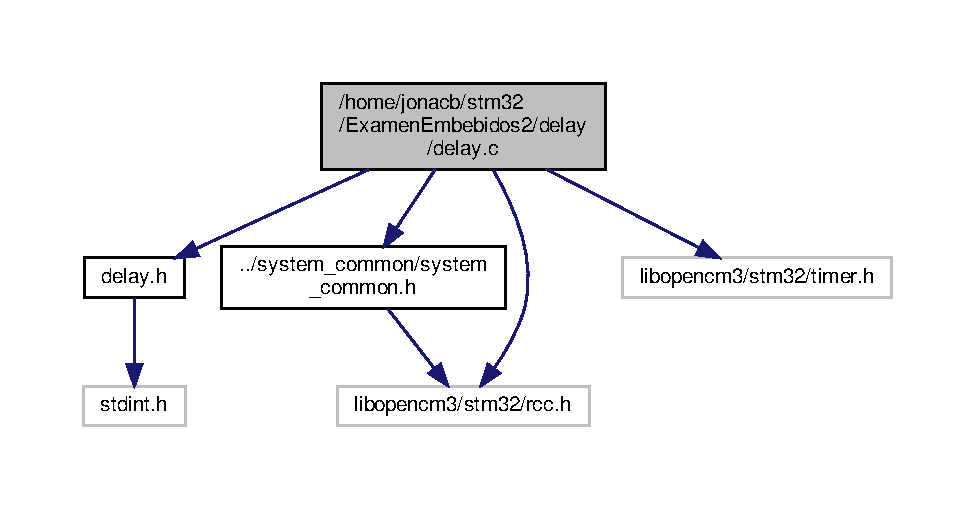
\includegraphics[width=350pt]{delay_8c__incl}
\end{center}
\end{figure}
\subsection*{Functions}
\begin{DoxyCompactItemize}
\item 
void \hyperlink{delay_8c_a820fbc8d56c8751e2c90dae94491c5de}{delay\+\_\+setup} (void)
\item 
void \hyperlink{delay_8c_ab7cce8122024d7ba47bf10f434956de4}{delay\+\_\+ms} (uint32\+\_\+t ms)
\end{DoxyCompactItemize}


\subsection{Detailed Description}
delay functions definitions. 



\subsection{Function Documentation}
\mbox{\Hypertarget{delay_8c_ab7cce8122024d7ba47bf10f434956de4}\label{delay_8c_ab7cce8122024d7ba47bf10f434956de4}} 
\index{delay.\+c@{delay.\+c}!delay\+\_\+ms@{delay\+\_\+ms}}
\index{delay\+\_\+ms@{delay\+\_\+ms}!delay.\+c@{delay.\+c}}
\subsubsection{\texorpdfstring{delay\+\_\+ms()}{delay\_ms()}}
{\footnotesize\ttfamily void delay\+\_\+ms (\begin{DoxyParamCaption}\item[{uint32\+\_\+t}]{ms }\end{DoxyParamCaption})}

Stablishes a delay in ms 
\begin{DoxyParams}[1]{Parameters}
\mbox{\tt in}  & {\em ms} & \\
\hline
\end{DoxyParams}
\mbox{\Hypertarget{delay_8c_a820fbc8d56c8751e2c90dae94491c5de}\label{delay_8c_a820fbc8d56c8751e2c90dae94491c5de}} 
\index{delay.\+c@{delay.\+c}!delay\+\_\+setup@{delay\+\_\+setup}}
\index{delay\+\_\+setup@{delay\+\_\+setup}!delay.\+c@{delay.\+c}}
\subsubsection{\texorpdfstring{delay\+\_\+setup()}{delay\_setup()}}
{\footnotesize\ttfamily void delay\+\_\+setup (\begin{DoxyParamCaption}\item[{void}]{ }\end{DoxyParamCaption})}

Sets up the timer used for the delay. 
\hypertarget{delay_8h}{}\section{/home/jonacb/stm32/\+Examen\+Embebidos2/delay/delay.h File Reference}
\label{delay_8h}\index{/home/jonacb/stm32/\+Examen\+Embebidos2/delay/delay.\+h@{/home/jonacb/stm32/\+Examen\+Embebidos2/delay/delay.\+h}}


delay header file.  


{\ttfamily \#include $<$stdint.\+h$>$}\newline
Include dependency graph for delay.\+h\+:\nopagebreak
\begin{figure}[H]
\begin{center}
\leavevmode
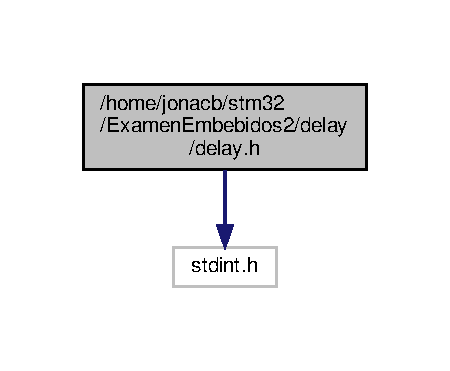
\includegraphics[width=216pt]{delay_8h__incl}
\end{center}
\end{figure}
This graph shows which files directly or indirectly include this file\+:\nopagebreak
\begin{figure}[H]
\begin{center}
\leavevmode
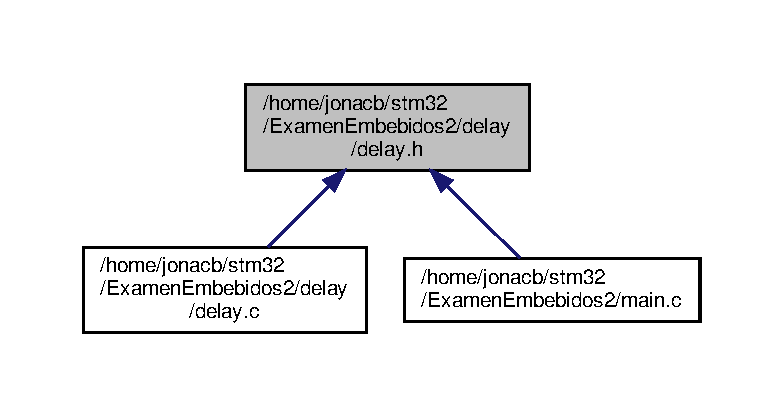
\includegraphics[width=350pt]{delay_8h__dep__incl}
\end{center}
\end{figure}
\subsection*{Functions}
\begin{DoxyCompactItemize}
\item 
void \hyperlink{delay_8h_a820fbc8d56c8751e2c90dae94491c5de}{delay\+\_\+setup} (void)
\item 
void \hyperlink{delay_8h_ab7cce8122024d7ba47bf10f434956de4}{delay\+\_\+ms} (uint32\+\_\+t ms)
\end{DoxyCompactItemize}


\subsection{Detailed Description}
delay header file. 



\subsection{Function Documentation}
\mbox{\Hypertarget{delay_8h_ab7cce8122024d7ba47bf10f434956de4}\label{delay_8h_ab7cce8122024d7ba47bf10f434956de4}} 
\index{delay.\+h@{delay.\+h}!delay\+\_\+ms@{delay\+\_\+ms}}
\index{delay\+\_\+ms@{delay\+\_\+ms}!delay.\+h@{delay.\+h}}
\subsubsection{\texorpdfstring{delay\+\_\+ms()}{delay\_ms()}}
{\footnotesize\ttfamily void delay\+\_\+ms (\begin{DoxyParamCaption}\item[{uint32\+\_\+t}]{ms }\end{DoxyParamCaption})}

Stablishes a delay in ms 
\begin{DoxyParams}[1]{Parameters}
\mbox{\tt in}  & {\em ms} & \\
\hline
\end{DoxyParams}
\mbox{\Hypertarget{delay_8h_a820fbc8d56c8751e2c90dae94491c5de}\label{delay_8h_a820fbc8d56c8751e2c90dae94491c5de}} 
\index{delay.\+h@{delay.\+h}!delay\+\_\+setup@{delay\+\_\+setup}}
\index{delay\+\_\+setup@{delay\+\_\+setup}!delay.\+h@{delay.\+h}}
\subsubsection{\texorpdfstring{delay\+\_\+setup()}{delay\_setup()}}
{\footnotesize\ttfamily void delay\+\_\+setup (\begin{DoxyParamCaption}\item[{void}]{ }\end{DoxyParamCaption})}

Sets up the timer used for the delay. 
\hypertarget{gpio_8c}{}\section{/home/jonacb/stm32/\+Examen\+Embebidos2/gpio/gpio.c File Reference}
\label{gpio_8c}\index{/home/jonacb/stm32/\+Examen\+Embebidos2/gpio/gpio.\+c@{/home/jonacb/stm32/\+Examen\+Embebidos2/gpio/gpio.\+c}}


G\+P\+IO function definitions.  


{\ttfamily \#include \char`\"{}gpio.\+h\char`\"{}}\newline
{\ttfamily \#include $<$libopencm3/stm32/rcc.\+h$>$}\newline
{\ttfamily \#include $<$libopencm3/stm32/gpio.\+h$>$}\newline
{\ttfamily \#include $<$stdint.\+h$>$}\newline
Include dependency graph for gpio.\+c\+:\nopagebreak
\begin{figure}[H]
\begin{center}
\leavevmode
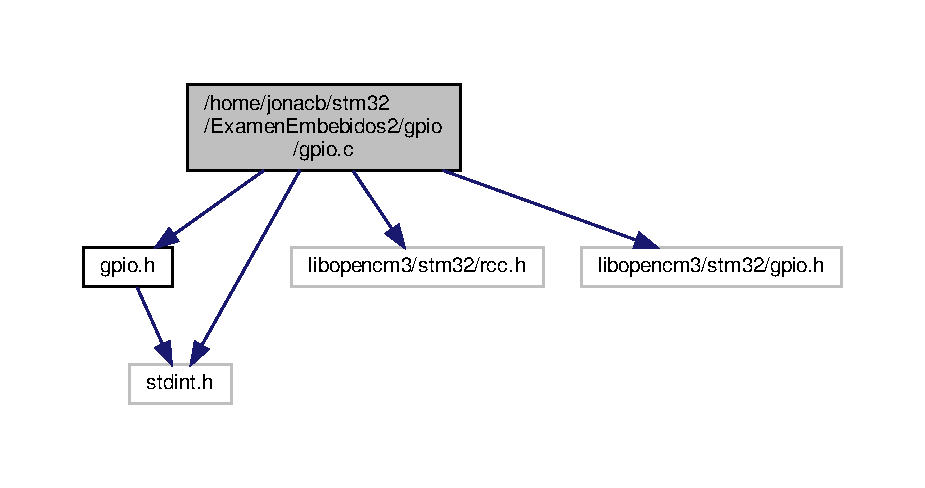
\includegraphics[width=350pt]{gpio_8c__incl}
\end{center}
\end{figure}
\subsection*{Functions}
\begin{DoxyCompactItemize}
\item 
void \hyperlink{gpio_8c_a5f93ca5922d03066040a1d1a96f22b50}{gpio\+\_\+init\+\_\+pin} (uint32\+\_\+t port, uint32\+\_\+t pin, \hyperlink{gpio_8h_a4ce7befa70373167bad76d2d332bd457}{pin\+Mode\+Type} mode)
\begin{DoxyCompactList}\small\item\em $<$libopencm3 G\+P\+IO functions \end{DoxyCompactList}\item 
\hyperlink{gpio_8h_a86299681096e04133f7b7de159bbfa5f}{pin\+Status\+Type} \hyperlink{gpio_8c_aa2c485c31c4c6a6fee2b69431bca91e0}{gpio\+\_\+get\+\_\+pin\+\_\+status} (uint32\+\_\+t port, uint32\+\_\+t pin)
\begin{DoxyCompactList}\small\item\em Returns the pin status when called. \end{DoxyCompactList}\item 
void \hyperlink{gpio_8c_ae43fe46d3907010a51432bb0fb10bc08}{gpio\+\_\+pin\+\_\+toggle} (uint32\+\_\+t port, uint32\+\_\+t pin)
\begin{DoxyCompactList}\small\item\em Toggle a given G\+P\+IO pin. \end{DoxyCompactList}\item 
void \hyperlink{gpio_8c_a23cdd4156dd0a9e343f6cc7e9396d6a2}{gpio\+\_\+pin\+\_\+set} (uint32\+\_\+t port, uint32\+\_\+t pin)
\begin{DoxyCompactList}\small\item\em Set a given G\+P\+IO pin. \end{DoxyCompactList}\item 
void \hyperlink{gpio_8c_a1af626a71fd9a5c7e59c250815067f31}{gpio\+\_\+pin\+\_\+reset} (uint32\+\_\+t port, uint32\+\_\+t pin)
\begin{DoxyCompactList}\small\item\em Clear a given G\+P\+IO pin. \end{DoxyCompactList}\end{DoxyCompactItemize}


\subsection{Detailed Description}
G\+P\+IO function definitions. 



\subsection{Function Documentation}
\mbox{\Hypertarget{gpio_8c_aa2c485c31c4c6a6fee2b69431bca91e0}\label{gpio_8c_aa2c485c31c4c6a6fee2b69431bca91e0}} 
\index{gpio.\+c@{gpio.\+c}!gpio\+\_\+get\+\_\+pin\+\_\+status@{gpio\+\_\+get\+\_\+pin\+\_\+status}}
\index{gpio\+\_\+get\+\_\+pin\+\_\+status@{gpio\+\_\+get\+\_\+pin\+\_\+status}!gpio.\+c@{gpio.\+c}}
\subsubsection{\texorpdfstring{gpio\+\_\+get\+\_\+pin\+\_\+status()}{gpio\_get\_pin\_status()}}
{\footnotesize\ttfamily \hyperlink{gpio_8h_a86299681096e04133f7b7de159bbfa5f}{pin\+Status\+Type} gpio\+\_\+get\+\_\+pin\+\_\+status (\begin{DoxyParamCaption}\item[{uint32\+\_\+t}]{port,  }\item[{uint32\+\_\+t}]{pin }\end{DoxyParamCaption})}



Returns the pin status when called. 


\begin{DoxyParams}[1]{Parameters}
\mbox{\tt in}  & {\em port} & -\/ G\+P\+IO block port. \\
\hline
\mbox{\tt in}  & {\em pin} & -\/ G\+P\+IO pin port. \\
\hline
\end{DoxyParams}
\begin{DoxyReturn}{Returns}
pin\+Status -\/ Status of the given G\+P\+IO pin. 
\end{DoxyReturn}
\mbox{\Hypertarget{gpio_8c_a5f93ca5922d03066040a1d1a96f22b50}\label{gpio_8c_a5f93ca5922d03066040a1d1a96f22b50}} 
\index{gpio.\+c@{gpio.\+c}!gpio\+\_\+init\+\_\+pin@{gpio\+\_\+init\+\_\+pin}}
\index{gpio\+\_\+init\+\_\+pin@{gpio\+\_\+init\+\_\+pin}!gpio.\+c@{gpio.\+c}}
\subsubsection{\texorpdfstring{gpio\+\_\+init\+\_\+pin()}{gpio\_init\_pin()}}
{\footnotesize\ttfamily void gpio\+\_\+init\+\_\+pin (\begin{DoxyParamCaption}\item[{uint32\+\_\+t}]{port,  }\item[{uint32\+\_\+t}]{pin,  }\item[{\hyperlink{gpio_8h_a4ce7befa70373167bad76d2d332bd457}{pin\+Mode\+Type}}]{mode }\end{DoxyParamCaption})}



$<$libopencm3 G\+P\+IO functions 

$<$G\+P\+IO Header $<$libopencm3 R\+CC functions Initialize a given G\+P\+IO pin. 
\begin{DoxyParams}[1]{Parameters}
\mbox{\tt in}  & {\em port} & -\/ G\+P\+IO block port to be started \\
\hline
\mbox{\tt in}  & {\em pin} & -\/ G\+P\+IO pin to be started \\
\hline
\mbox{\tt in}  & {\em mode} & -\/ How will the pin be initialized $<$I\+N\+P\+U\+T/\+O\+U\+T\+P\+UT$>$ \\
\hline
\end{DoxyParams}
\mbox{\Hypertarget{gpio_8c_a1af626a71fd9a5c7e59c250815067f31}\label{gpio_8c_a1af626a71fd9a5c7e59c250815067f31}} 
\index{gpio.\+c@{gpio.\+c}!gpio\+\_\+pin\+\_\+reset@{gpio\+\_\+pin\+\_\+reset}}
\index{gpio\+\_\+pin\+\_\+reset@{gpio\+\_\+pin\+\_\+reset}!gpio.\+c@{gpio.\+c}}
\subsubsection{\texorpdfstring{gpio\+\_\+pin\+\_\+reset()}{gpio\_pin\_reset()}}
{\footnotesize\ttfamily void gpio\+\_\+pin\+\_\+reset (\begin{DoxyParamCaption}\item[{uint32\+\_\+t}]{port,  }\item[{uint32\+\_\+t}]{pin }\end{DoxyParamCaption})}



Clear a given G\+P\+IO pin. 


\begin{DoxyParams}[1]{Parameters}
\mbox{\tt in}  & {\em port} & -\/ G\+P\+IO block port. \\
\hline
\mbox{\tt in}  & {\em pin} & -\/ G\+P\+IO pin port. \\
\hline
\end{DoxyParams}
\mbox{\Hypertarget{gpio_8c_a23cdd4156dd0a9e343f6cc7e9396d6a2}\label{gpio_8c_a23cdd4156dd0a9e343f6cc7e9396d6a2}} 
\index{gpio.\+c@{gpio.\+c}!gpio\+\_\+pin\+\_\+set@{gpio\+\_\+pin\+\_\+set}}
\index{gpio\+\_\+pin\+\_\+set@{gpio\+\_\+pin\+\_\+set}!gpio.\+c@{gpio.\+c}}
\subsubsection{\texorpdfstring{gpio\+\_\+pin\+\_\+set()}{gpio\_pin\_set()}}
{\footnotesize\ttfamily void gpio\+\_\+pin\+\_\+set (\begin{DoxyParamCaption}\item[{uint32\+\_\+t}]{port,  }\item[{uint32\+\_\+t}]{pin }\end{DoxyParamCaption})}



Set a given G\+P\+IO pin. 


\begin{DoxyParams}[1]{Parameters}
\mbox{\tt in}  & {\em port} & -\/ G\+P\+IO block port. \\
\hline
\mbox{\tt in}  & {\em pin} & -\/ G\+P\+IO pin port. \\
\hline
\end{DoxyParams}
\mbox{\Hypertarget{gpio_8c_ae43fe46d3907010a51432bb0fb10bc08}\label{gpio_8c_ae43fe46d3907010a51432bb0fb10bc08}} 
\index{gpio.\+c@{gpio.\+c}!gpio\+\_\+pin\+\_\+toggle@{gpio\+\_\+pin\+\_\+toggle}}
\index{gpio\+\_\+pin\+\_\+toggle@{gpio\+\_\+pin\+\_\+toggle}!gpio.\+c@{gpio.\+c}}
\subsubsection{\texorpdfstring{gpio\+\_\+pin\+\_\+toggle()}{gpio\_pin\_toggle()}}
{\footnotesize\ttfamily void gpio\+\_\+pin\+\_\+toggle (\begin{DoxyParamCaption}\item[{uint32\+\_\+t}]{port,  }\item[{uint32\+\_\+t}]{pin }\end{DoxyParamCaption})}



Toggle a given G\+P\+IO pin. 


\begin{DoxyParams}[1]{Parameters}
\mbox{\tt in}  & {\em port} & -\/ G\+P\+IO block port. \\
\hline
\mbox{\tt in}  & {\em pin} & -\/ G\+P\+IO pin port. \\
\hline
\end{DoxyParams}

\hypertarget{gpio_8h}{}\section{/home/jonacb/stm32/\+Examen\+Embebidos2/gpio/gpio.h File Reference}
\label{gpio_8h}\index{/home/jonacb/stm32/\+Examen\+Embebidos2/gpio/gpio.\+h@{/home/jonacb/stm32/\+Examen\+Embebidos2/gpio/gpio.\+h}}


G\+P\+IO header file.  


{\ttfamily \#include $<$stdint.\+h$>$}\newline
Include dependency graph for gpio.\+h\+:\nopagebreak
\begin{figure}[H]
\begin{center}
\leavevmode
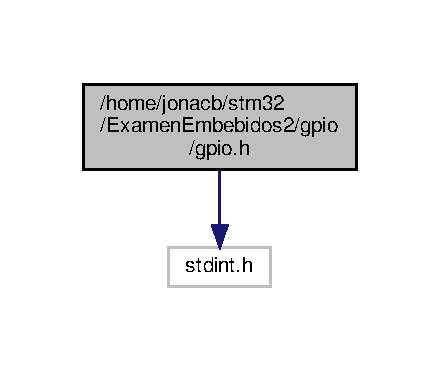
\includegraphics[width=211pt]{gpio_8h__incl}
\end{center}
\end{figure}
This graph shows which files directly or indirectly include this file\+:\nopagebreak
\begin{figure}[H]
\begin{center}
\leavevmode
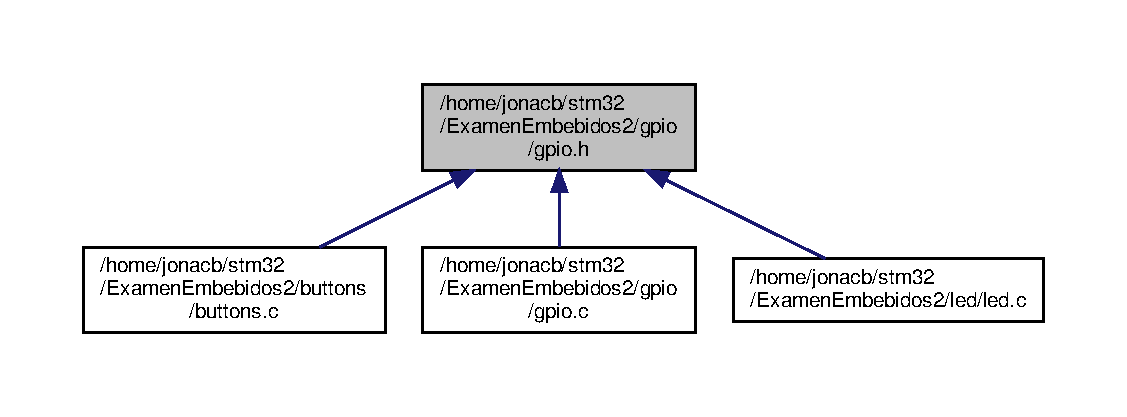
\includegraphics[width=350pt]{gpio_8h__dep__incl}
\end{center}
\end{figure}
\subsection*{Enumerations}
\begin{DoxyCompactItemize}
\item 
enum \hyperlink{gpio_8h_a4ce7befa70373167bad76d2d332bd457}{pin\+Mode\+Type} \{ \hyperlink{gpio_8h_a4ce7befa70373167bad76d2d332bd457ae310c909d76b003d016bef8bdf16936a}{I\+N\+P\+UT}, 
\hyperlink{gpio_8h_a4ce7befa70373167bad76d2d332bd457a2ab08d3e103968f5f4f26b66a52e99d6}{O\+U\+T\+P\+UT}
 \}\begin{DoxyCompactList}\small\item\em $<$stdint definitions. \end{DoxyCompactList}
\item 
enum \hyperlink{gpio_8h_a86299681096e04133f7b7de159bbfa5f}{pin\+Status\+Type} \{ \hyperlink{gpio_8h_a86299681096e04133f7b7de159bbfa5fab44c8101cc294c074709ec1b14211792}{S\+ET}, 
\hyperlink{gpio_8h_a86299681096e04133f7b7de159bbfa5fa589b7d94a3d91d145720e2fed0eb3a05}{R\+E\+S\+ET}
 \}\begin{DoxyCompactList}\small\item\em Enum class defining different pin status. \end{DoxyCompactList}
\end{DoxyCompactItemize}
\subsection*{Functions}
\begin{DoxyCompactItemize}
\item 
void \hyperlink{gpio_8h_a5f93ca5922d03066040a1d1a96f22b50}{gpio\+\_\+init\+\_\+pin} (uint32\+\_\+t port, uint32\+\_\+t pin, \hyperlink{gpio_8h_a4ce7befa70373167bad76d2d332bd457}{pin\+Mode\+Type} mode)
\begin{DoxyCompactList}\small\item\em $<$libopencm3 G\+P\+IO functions \end{DoxyCompactList}\item 
\hyperlink{gpio_8h_a86299681096e04133f7b7de159bbfa5f}{pin\+Status\+Type} \hyperlink{gpio_8h_aa2c485c31c4c6a6fee2b69431bca91e0}{gpio\+\_\+get\+\_\+pin\+\_\+status} (uint32\+\_\+t port, uint32\+\_\+t pin)
\begin{DoxyCompactList}\small\item\em Returns the pin status when called. \end{DoxyCompactList}\item 
void \hyperlink{gpio_8h_ae43fe46d3907010a51432bb0fb10bc08}{gpio\+\_\+pin\+\_\+toggle} (uint32\+\_\+t port, uint32\+\_\+t pin)
\begin{DoxyCompactList}\small\item\em Toggle a given G\+P\+IO pin. \end{DoxyCompactList}\item 
void \hyperlink{gpio_8h_a23cdd4156dd0a9e343f6cc7e9396d6a2}{gpio\+\_\+pin\+\_\+set} (uint32\+\_\+t port, uint32\+\_\+t pin)
\begin{DoxyCompactList}\small\item\em Set a given G\+P\+IO pin. \end{DoxyCompactList}\item 
void \hyperlink{gpio_8h_a1af626a71fd9a5c7e59c250815067f31}{gpio\+\_\+pin\+\_\+reset} (uint32\+\_\+t port, uint32\+\_\+t pin)
\begin{DoxyCompactList}\small\item\em Clear a given G\+P\+IO pin. \end{DoxyCompactList}\end{DoxyCompactItemize}


\subsection{Detailed Description}
G\+P\+IO header file. 



\subsection{Enumeration Type Documentation}
\mbox{\Hypertarget{gpio_8h_a4ce7befa70373167bad76d2d332bd457}\label{gpio_8h_a4ce7befa70373167bad76d2d332bd457}} 
\index{gpio.\+h@{gpio.\+h}!pin\+Mode\+Type@{pin\+Mode\+Type}}
\index{pin\+Mode\+Type@{pin\+Mode\+Type}!gpio.\+h@{gpio.\+h}}
\subsubsection{\texorpdfstring{pin\+Mode\+Type}{pinModeType}}
{\footnotesize\ttfamily enum \hyperlink{gpio_8h_a4ce7befa70373167bad76d2d332bd457}{pin\+Mode\+Type}}



$<$stdint definitions. 

Enum class defining the pin mode. \begin{DoxyEnumFields}{Enumerator}
\raisebox{\heightof{T}}[0pt][0pt]{\index{I\+N\+P\+UT@{I\+N\+P\+UT}!gpio.\+h@{gpio.\+h}}\index{gpio.\+h@{gpio.\+h}!I\+N\+P\+UT@{I\+N\+P\+UT}}}\mbox{\Hypertarget{gpio_8h_a4ce7befa70373167bad76d2d332bd457ae310c909d76b003d016bef8bdf16936a}\label{gpio_8h_a4ce7befa70373167bad76d2d332bd457ae310c909d76b003d016bef8bdf16936a}} 
I\+N\+P\+UT&Input mode. \\
\hline

\raisebox{\heightof{T}}[0pt][0pt]{\index{O\+U\+T\+P\+UT@{O\+U\+T\+P\+UT}!gpio.\+h@{gpio.\+h}}\index{gpio.\+h@{gpio.\+h}!O\+U\+T\+P\+UT@{O\+U\+T\+P\+UT}}}\mbox{\Hypertarget{gpio_8h_a4ce7befa70373167bad76d2d332bd457a2ab08d3e103968f5f4f26b66a52e99d6}\label{gpio_8h_a4ce7befa70373167bad76d2d332bd457a2ab08d3e103968f5f4f26b66a52e99d6}} 
O\+U\+T\+P\+UT&Output mode. \\
\hline

\end{DoxyEnumFields}
\mbox{\Hypertarget{gpio_8h_a86299681096e04133f7b7de159bbfa5f}\label{gpio_8h_a86299681096e04133f7b7de159bbfa5f}} 
\index{gpio.\+h@{gpio.\+h}!pin\+Status\+Type@{pin\+Status\+Type}}
\index{pin\+Status\+Type@{pin\+Status\+Type}!gpio.\+h@{gpio.\+h}}
\subsubsection{\texorpdfstring{pin\+Status\+Type}{pinStatusType}}
{\footnotesize\ttfamily enum \hyperlink{gpio_8h_a86299681096e04133f7b7de159bbfa5f}{pin\+Status\+Type}}



Enum class defining different pin status. 

\begin{DoxyEnumFields}{Enumerator}
\raisebox{\heightof{T}}[0pt][0pt]{\index{S\+ET@{S\+ET}!gpio.\+h@{gpio.\+h}}\index{gpio.\+h@{gpio.\+h}!S\+ET@{S\+ET}}}\mbox{\Hypertarget{gpio_8h_a86299681096e04133f7b7de159bbfa5fab44c8101cc294c074709ec1b14211792}\label{gpio_8h_a86299681096e04133f7b7de159bbfa5fab44c8101cc294c074709ec1b14211792}} 
S\+ET&Pin is set. \\
\hline

\raisebox{\heightof{T}}[0pt][0pt]{\index{R\+E\+S\+ET@{R\+E\+S\+ET}!gpio.\+h@{gpio.\+h}}\index{gpio.\+h@{gpio.\+h}!R\+E\+S\+ET@{R\+E\+S\+ET}}}\mbox{\Hypertarget{gpio_8h_a86299681096e04133f7b7de159bbfa5fa589b7d94a3d91d145720e2fed0eb3a05}\label{gpio_8h_a86299681096e04133f7b7de159bbfa5fa589b7d94a3d91d145720e2fed0eb3a05}} 
R\+E\+S\+ET&Pin is cleared. \\
\hline

\end{DoxyEnumFields}


\subsection{Function Documentation}
\mbox{\Hypertarget{gpio_8h_aa2c485c31c4c6a6fee2b69431bca91e0}\label{gpio_8h_aa2c485c31c4c6a6fee2b69431bca91e0}} 
\index{gpio.\+h@{gpio.\+h}!gpio\+\_\+get\+\_\+pin\+\_\+status@{gpio\+\_\+get\+\_\+pin\+\_\+status}}
\index{gpio\+\_\+get\+\_\+pin\+\_\+status@{gpio\+\_\+get\+\_\+pin\+\_\+status}!gpio.\+h@{gpio.\+h}}
\subsubsection{\texorpdfstring{gpio\+\_\+get\+\_\+pin\+\_\+status()}{gpio\_get\_pin\_status()}}
{\footnotesize\ttfamily \hyperlink{gpio_8h_a86299681096e04133f7b7de159bbfa5f}{pin\+Status\+Type} gpio\+\_\+get\+\_\+pin\+\_\+status (\begin{DoxyParamCaption}\item[{uint32\+\_\+t}]{port,  }\item[{uint32\+\_\+t}]{pin }\end{DoxyParamCaption})}



Returns the pin status when called. 


\begin{DoxyParams}[1]{Parameters}
\mbox{\tt in}  & {\em port} & -\/ G\+P\+IO block port. \\
\hline
\mbox{\tt in}  & {\em pin} & -\/ G\+P\+IO pin port. \\
\hline
\end{DoxyParams}
\begin{DoxyReturn}{Returns}
pin\+Status -\/ Status of the given G\+P\+IO pin. 
\end{DoxyReturn}
\mbox{\Hypertarget{gpio_8h_a5f93ca5922d03066040a1d1a96f22b50}\label{gpio_8h_a5f93ca5922d03066040a1d1a96f22b50}} 
\index{gpio.\+h@{gpio.\+h}!gpio\+\_\+init\+\_\+pin@{gpio\+\_\+init\+\_\+pin}}
\index{gpio\+\_\+init\+\_\+pin@{gpio\+\_\+init\+\_\+pin}!gpio.\+h@{gpio.\+h}}
\subsubsection{\texorpdfstring{gpio\+\_\+init\+\_\+pin()}{gpio\_init\_pin()}}
{\footnotesize\ttfamily void gpio\+\_\+init\+\_\+pin (\begin{DoxyParamCaption}\item[{uint32\+\_\+t}]{port,  }\item[{uint32\+\_\+t}]{pin,  }\item[{\hyperlink{gpio_8h_a4ce7befa70373167bad76d2d332bd457}{pin\+Mode\+Type}}]{mode }\end{DoxyParamCaption})}



$<$libopencm3 G\+P\+IO functions 

$<$G\+P\+IO Header $<$libopencm3 R\+CC functions Initialize a given G\+P\+IO pin. 
\begin{DoxyParams}[1]{Parameters}
\mbox{\tt in}  & {\em port} & -\/ G\+P\+IO block port to be started \\
\hline
\mbox{\tt in}  & {\em pin} & -\/ G\+P\+IO pin to be started \\
\hline
\mbox{\tt in}  & {\em mode} & -\/ How will the pin be initialized $<$I\+N\+P\+U\+T/\+O\+U\+T\+P\+UT$>$ \\
\hline
\end{DoxyParams}
\mbox{\Hypertarget{gpio_8h_a1af626a71fd9a5c7e59c250815067f31}\label{gpio_8h_a1af626a71fd9a5c7e59c250815067f31}} 
\index{gpio.\+h@{gpio.\+h}!gpio\+\_\+pin\+\_\+reset@{gpio\+\_\+pin\+\_\+reset}}
\index{gpio\+\_\+pin\+\_\+reset@{gpio\+\_\+pin\+\_\+reset}!gpio.\+h@{gpio.\+h}}
\subsubsection{\texorpdfstring{gpio\+\_\+pin\+\_\+reset()}{gpio\_pin\_reset()}}
{\footnotesize\ttfamily void gpio\+\_\+pin\+\_\+reset (\begin{DoxyParamCaption}\item[{uint32\+\_\+t}]{port,  }\item[{uint32\+\_\+t}]{pin }\end{DoxyParamCaption})}



Clear a given G\+P\+IO pin. 


\begin{DoxyParams}[1]{Parameters}
\mbox{\tt in}  & {\em port} & -\/ G\+P\+IO block port. \\
\hline
\mbox{\tt in}  & {\em pin} & -\/ G\+P\+IO pin port. \\
\hline
\end{DoxyParams}
\mbox{\Hypertarget{gpio_8h_a23cdd4156dd0a9e343f6cc7e9396d6a2}\label{gpio_8h_a23cdd4156dd0a9e343f6cc7e9396d6a2}} 
\index{gpio.\+h@{gpio.\+h}!gpio\+\_\+pin\+\_\+set@{gpio\+\_\+pin\+\_\+set}}
\index{gpio\+\_\+pin\+\_\+set@{gpio\+\_\+pin\+\_\+set}!gpio.\+h@{gpio.\+h}}
\subsubsection{\texorpdfstring{gpio\+\_\+pin\+\_\+set()}{gpio\_pin\_set()}}
{\footnotesize\ttfamily void gpio\+\_\+pin\+\_\+set (\begin{DoxyParamCaption}\item[{uint32\+\_\+t}]{port,  }\item[{uint32\+\_\+t}]{pin }\end{DoxyParamCaption})}



Set a given G\+P\+IO pin. 


\begin{DoxyParams}[1]{Parameters}
\mbox{\tt in}  & {\em port} & -\/ G\+P\+IO block port. \\
\hline
\mbox{\tt in}  & {\em pin} & -\/ G\+P\+IO pin port. \\
\hline
\end{DoxyParams}
\mbox{\Hypertarget{gpio_8h_ae43fe46d3907010a51432bb0fb10bc08}\label{gpio_8h_ae43fe46d3907010a51432bb0fb10bc08}} 
\index{gpio.\+h@{gpio.\+h}!gpio\+\_\+pin\+\_\+toggle@{gpio\+\_\+pin\+\_\+toggle}}
\index{gpio\+\_\+pin\+\_\+toggle@{gpio\+\_\+pin\+\_\+toggle}!gpio.\+h@{gpio.\+h}}
\subsubsection{\texorpdfstring{gpio\+\_\+pin\+\_\+toggle()}{gpio\_pin\_toggle()}}
{\footnotesize\ttfamily void gpio\+\_\+pin\+\_\+toggle (\begin{DoxyParamCaption}\item[{uint32\+\_\+t}]{port,  }\item[{uint32\+\_\+t}]{pin }\end{DoxyParamCaption})}



Toggle a given G\+P\+IO pin. 


\begin{DoxyParams}[1]{Parameters}
\mbox{\tt in}  & {\em port} & -\/ G\+P\+IO block port. \\
\hline
\mbox{\tt in}  & {\em pin} & -\/ G\+P\+IO pin port. \\
\hline
\end{DoxyParams}

\hypertarget{led_8c}{}\section{/home/jonacb/stm32/\+Examen\+Embebidos2/led/led.c File Reference}
\label{led_8c}\index{/home/jonacb/stm32/\+Examen\+Embebidos2/led/led.\+c@{/home/jonacb/stm32/\+Examen\+Embebidos2/led/led.\+c}}


Defines L\+ED functions.  


{\ttfamily \#include \char`\"{}led.\+h\char`\"{}}\newline
{\ttfamily \#include \char`\"{}../gpio/gpio.\+h\char`\"{}}\newline
Include dependency graph for led.\+c\+:\nopagebreak
\begin{figure}[H]
\begin{center}
\leavevmode
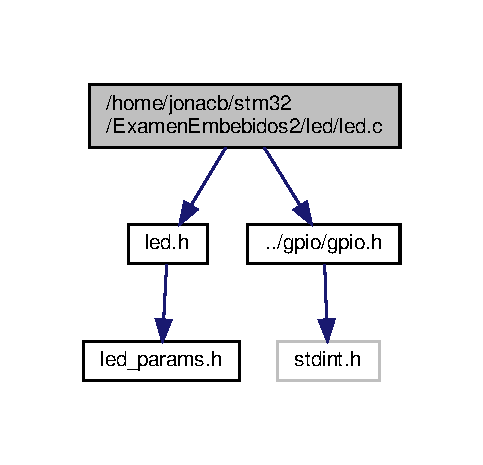
\includegraphics[width=232pt]{led_8c__incl}
\end{center}
\end{figure}
\subsection*{Functions}
\begin{DoxyCompactItemize}
\item 
void \hyperlink{led_8c_a45a4dce2a793aa9be79132acc6527869}{led\+\_\+setup} (void)
\begin{DoxyCompactList}\small\item\em Sets up the L\+ED port and pins. \end{DoxyCompactList}\item 
\mbox{\Hypertarget{led_8c_a487f9f3640c7f6b9b416134274259866}\label{led_8c_a487f9f3640c7f6b9b416134274259866}} 
void \hyperlink{led_8c_a487f9f3640c7f6b9b416134274259866}{led\+\_\+toggle} (void)
\begin{DoxyCompactList}\small\item\em Toggles the L\+ED. \end{DoxyCompactList}\item 
\mbox{\Hypertarget{led_8c_a801936b261245054eb570e040642818a}\label{led_8c_a801936b261245054eb570e040642818a}} 
void \hyperlink{led_8c_a801936b261245054eb570e040642818a}{led\+\_\+on} (void)
\begin{DoxyCompactList}\small\item\em Turns on the L\+ED. \end{DoxyCompactList}\item 
\mbox{\Hypertarget{led_8c_a429f05b7eac928971c19e37ddc7079be}\label{led_8c_a429f05b7eac928971c19e37ddc7079be}} 
void \hyperlink{led_8c_a429f05b7eac928971c19e37ddc7079be}{led\+\_\+off} (void)
\begin{DoxyCompactList}\small\item\em Turns off the L\+ED. \end{DoxyCompactList}\end{DoxyCompactItemize}


\subsection{Detailed Description}
Defines L\+ED functions. 



\subsection{Function Documentation}
\mbox{\Hypertarget{led_8c_a45a4dce2a793aa9be79132acc6527869}\label{led_8c_a45a4dce2a793aa9be79132acc6527869}} 
\index{led.\+c@{led.\+c}!led\+\_\+setup@{led\+\_\+setup}}
\index{led\+\_\+setup@{led\+\_\+setup}!led.\+c@{led.\+c}}
\subsubsection{\texorpdfstring{led\+\_\+setup()}{led\_setup()}}
{\footnotesize\ttfamily void led\+\_\+setup (\begin{DoxyParamCaption}\item[{void}]{ }\end{DoxyParamCaption})}



Sets up the L\+ED port and pins. 

$<$L\+ED params header include. 
\hypertarget{led_8h}{}\section{/home/jonacb/stm32/\+Examen\+Embebidos2/led/led.h File Reference}
\label{led_8h}\index{/home/jonacb/stm32/\+Examen\+Embebidos2/led/led.\+h@{/home/jonacb/stm32/\+Examen\+Embebidos2/led/led.\+h}}


L\+ED header file.  


{\ttfamily \#include \char`\"{}led\+\_\+params.\+h\char`\"{}}\newline
Include dependency graph for led.\+h\+:\nopagebreak
\begin{figure}[H]
\begin{center}
\leavevmode
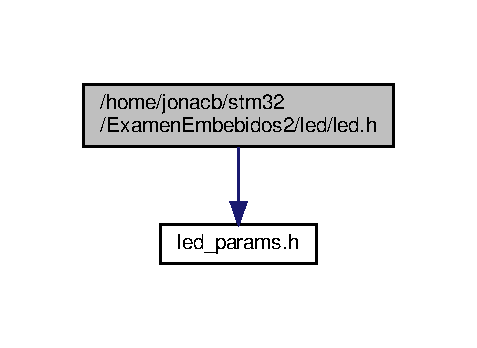
\includegraphics[width=229pt]{led_8h__incl}
\end{center}
\end{figure}
This graph shows which files directly or indirectly include this file\+:\nopagebreak
\begin{figure}[H]
\begin{center}
\leavevmode
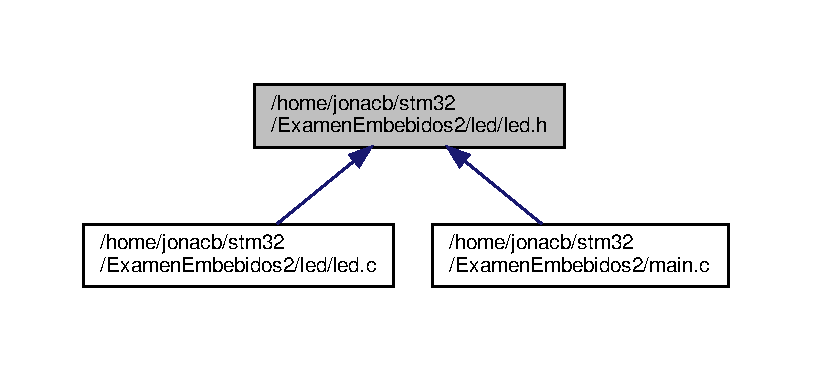
\includegraphics[width=350pt]{led_8h__dep__incl}
\end{center}
\end{figure}
\subsection*{Functions}
\begin{DoxyCompactItemize}
\item 
void \hyperlink{led_8h_a45a4dce2a793aa9be79132acc6527869}{led\+\_\+setup} (void)
\begin{DoxyCompactList}\small\item\em $<$L\+ED params header include. \end{DoxyCompactList}\item 
\mbox{\Hypertarget{led_8h_a487f9f3640c7f6b9b416134274259866}\label{led_8h_a487f9f3640c7f6b9b416134274259866}} 
void \hyperlink{led_8h_a487f9f3640c7f6b9b416134274259866}{led\+\_\+toggle} (void)
\begin{DoxyCompactList}\small\item\em Toggles the L\+ED. \end{DoxyCompactList}\item 
\mbox{\Hypertarget{led_8h_a801936b261245054eb570e040642818a}\label{led_8h_a801936b261245054eb570e040642818a}} 
void \hyperlink{led_8h_a801936b261245054eb570e040642818a}{led\+\_\+on} (void)
\begin{DoxyCompactList}\small\item\em Turns on the L\+ED. \end{DoxyCompactList}\item 
\mbox{\Hypertarget{led_8h_a429f05b7eac928971c19e37ddc7079be}\label{led_8h_a429f05b7eac928971c19e37ddc7079be}} 
void \hyperlink{led_8h_a429f05b7eac928971c19e37ddc7079be}{led\+\_\+off} (void)
\begin{DoxyCompactList}\small\item\em Turns off the L\+ED. \end{DoxyCompactList}\end{DoxyCompactItemize}


\subsection{Detailed Description}
L\+ED header file. 



\subsection{Function Documentation}
\mbox{\Hypertarget{led_8h_a45a4dce2a793aa9be79132acc6527869}\label{led_8h_a45a4dce2a793aa9be79132acc6527869}} 
\index{led.\+h@{led.\+h}!led\+\_\+setup@{led\+\_\+setup}}
\index{led\+\_\+setup@{led\+\_\+setup}!led.\+h@{led.\+h}}
\subsubsection{\texorpdfstring{led\+\_\+setup()}{led\_setup()}}
{\footnotesize\ttfamily void led\+\_\+setup (\begin{DoxyParamCaption}\item[{void}]{ }\end{DoxyParamCaption})}



$<$L\+ED params header include. 

$<$L\+ED params header include. 
\hypertarget{led__params_8h}{}\section{/home/jonacb/stm32/\+Examen\+Embebidos2/led/led\+\_\+params.h File Reference}
\label{led__params_8h}\index{/home/jonacb/stm32/\+Examen\+Embebidos2/led/led\+\_\+params.\+h@{/home/jonacb/stm32/\+Examen\+Embebidos2/led/led\+\_\+params.\+h}}


L\+ED P\+A\+R\+A\+MS N\+E\+E\+D\+ED.  


This graph shows which files directly or indirectly include this file\+:\nopagebreak
\begin{figure}[H]
\begin{center}
\leavevmode
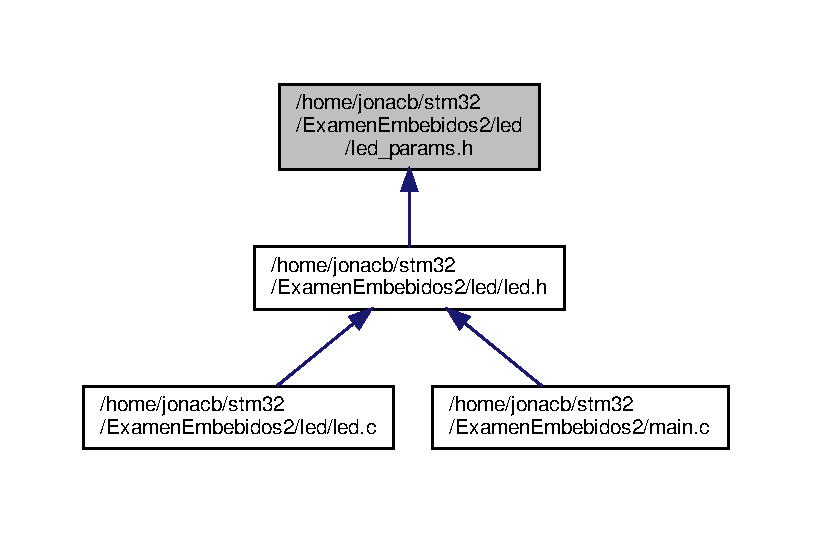
\includegraphics[width=350pt]{led__params_8h__dep__incl}
\end{center}
\end{figure}
\subsection*{Macros}
\begin{DoxyCompactItemize}
\item 
\mbox{\Hypertarget{led__params_8h_a663daa01e565aee93c6f20c5845b90b4}\label{led__params_8h_a663daa01e565aee93c6f20c5845b90b4}} 
\#define \hyperlink{led__params_8h_a663daa01e565aee93c6f20c5845b90b4}{L\+E\+D\+\_\+\+P\+O\+RT}~1
\begin{DoxyCompactList}\small\item\em L\+ED port to be used. \end{DoxyCompactList}\item 
\mbox{\Hypertarget{led__params_8h_ab4553be4db9860d940f81d7447173b2f}\label{led__params_8h_ab4553be4db9860d940f81d7447173b2f}} 
\#define \hyperlink{led__params_8h_ab4553be4db9860d940f81d7447173b2f}{L\+E\+D\+\_\+\+P\+IN}~1
\begin{DoxyCompactList}\small\item\em L\+ED pin to be used. \end{DoxyCompactList}\end{DoxyCompactItemize}


\subsection{Detailed Description}
L\+ED P\+A\+R\+A\+MS N\+E\+E\+D\+ED. 


\hypertarget{main_8c}{}\section{/home/jonacb/stm32/\+Examen\+Embebidos2/main.c File Reference}
\label{main_8c}\index{/home/jonacb/stm32/\+Examen\+Embebidos2/main.\+c@{/home/jonacb/stm32/\+Examen\+Embebidos2/main.\+c}}


Main code for this project.  


{\ttfamily \#include \char`\"{}system\+\_\+common/system\+\_\+common.\+h\char`\"{}}\newline
{\ttfamily \#include \char`\"{}timer/timer.\+h\char`\"{}}\newline
{\ttfamily \#include \char`\"{}delay/delay.\+h\char`\"{}}\newline
{\ttfamily \#include \char`\"{}print/print.\+h\char`\"{}}\newline
{\ttfamily \#include \char`\"{}buttons/buttons.\+h\char`\"{}}\newline
{\ttfamily \#include \char`\"{}led/led.\+h\char`\"{}}\newline
Include dependency graph for main.\+c\+:\nopagebreak
\begin{figure}[H]
\begin{center}
\leavevmode
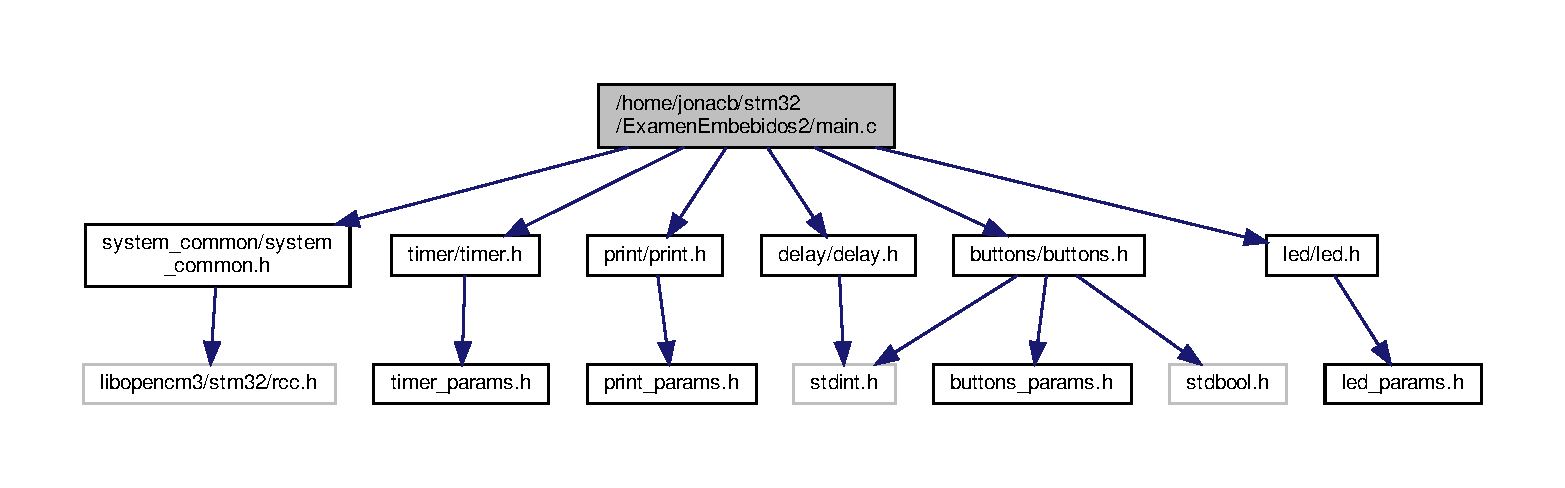
\includegraphics[width=350pt]{main_8c__incl}
\end{center}
\end{figure}
\subsection*{Enumerations}
\begin{DoxyCompactItemize}
\item 
enum \hyperlink{main_8c_a4a3a6e72418c2bb8d8b1ce55c1a655c0}{timer\+Status\+Type} \{ \hyperlink{main_8c_a4a3a6e72418c2bb8d8b1ce55c1a655c0aac132f2982b98bcaa3445e535a03ff75}{O\+FF}, 
\hyperlink{main_8c_a4a3a6e72418c2bb8d8b1ce55c1a655c0a1061be6c3fb88d32829cba6f6b2be304}{R\+U\+N\+N\+I\+NG}, 
\hyperlink{main_8c_a4a3a6e72418c2bb8d8b1ce55c1a655c0ad4bb05915de3c370d3a33d4f51389655}{P\+A\+U\+S\+ED}
 \}\begin{DoxyCompactList}\small\item\em $<$System common defines. \end{DoxyCompactList}
\end{DoxyCompactItemize}
\subsection*{Functions}
\begin{DoxyCompactItemize}
\item 
\mbox{\Hypertarget{main_8c_a840291bc02cba5474a4cb46a9b9566fe}\label{main_8c_a840291bc02cba5474a4cb46a9b9566fe}} 
int \hyperlink{main_8c_a840291bc02cba5474a4cb46a9b9566fe}{main} (void)
\begin{DoxyCompactList}\small\item\em Main function. \end{DoxyCompactList}\end{DoxyCompactItemize}
\subsection*{Variables}
\begin{DoxyCompactItemize}
\item 
\mbox{\Hypertarget{main_8c_a722c7add7953a03d0f6dcc1a67aba2cd}\label{main_8c_a722c7add7953a03d0f6dcc1a67aba2cd}} 
\hyperlink{main_8c_a4a3a6e72418c2bb8d8b1ce55c1a655c0}{timer\+Status\+Type} \hyperlink{main_8c_a722c7add7953a03d0f6dcc1a67aba2cd}{timer\+\_\+status} = \hyperlink{main_8c_a4a3a6e72418c2bb8d8b1ce55c1a655c0aac132f2982b98bcaa3445e535a03ff75}{O\+FF}
\begin{DoxyCompactList}\small\item\em Timer default status. \end{DoxyCompactList}\end{DoxyCompactItemize}


\subsection{Detailed Description}
Main code for this project. 



\subsection{Enumeration Type Documentation}
\mbox{\Hypertarget{main_8c_a4a3a6e72418c2bb8d8b1ce55c1a655c0}\label{main_8c_a4a3a6e72418c2bb8d8b1ce55c1a655c0}} 
\index{main.\+c@{main.\+c}!timer\+Status\+Type@{timer\+Status\+Type}}
\index{timer\+Status\+Type@{timer\+Status\+Type}!main.\+c@{main.\+c}}
\subsubsection{\texorpdfstring{timer\+Status\+Type}{timerStatusType}}
{\footnotesize\ttfamily enum \hyperlink{main_8c_a4a3a6e72418c2bb8d8b1ce55c1a655c0}{timer\+Status\+Type}}



$<$System common defines. 

$<$Delay header file include. $<$Button header file include. L\+ED header file include. Enum class defining the timer status. \begin{DoxyEnumFields}{Enumerator}
\raisebox{\heightof{T}}[0pt][0pt]{\index{O\+FF@{O\+FF}!main.\+c@{main.\+c}}\index{main.\+c@{main.\+c}!O\+FF@{O\+FF}}}\mbox{\Hypertarget{main_8c_a4a3a6e72418c2bb8d8b1ce55c1a655c0aac132f2982b98bcaa3445e535a03ff75}\label{main_8c_a4a3a6e72418c2bb8d8b1ce55c1a655c0aac132f2982b98bcaa3445e535a03ff75}} 
O\+FF&Timer is off. \\
\hline

\raisebox{\heightof{T}}[0pt][0pt]{\index{R\+U\+N\+N\+I\+NG@{R\+U\+N\+N\+I\+NG}!main.\+c@{main.\+c}}\index{main.\+c@{main.\+c}!R\+U\+N\+N\+I\+NG@{R\+U\+N\+N\+I\+NG}}}\mbox{\Hypertarget{main_8c_a4a3a6e72418c2bb8d8b1ce55c1a655c0a1061be6c3fb88d32829cba6f6b2be304}\label{main_8c_a4a3a6e72418c2bb8d8b1ce55c1a655c0a1061be6c3fb88d32829cba6f6b2be304}} 
R\+U\+N\+N\+I\+NG&Timer is running. \\
\hline

\raisebox{\heightof{T}}[0pt][0pt]{\index{P\+A\+U\+S\+ED@{P\+A\+U\+S\+ED}!main.\+c@{main.\+c}}\index{main.\+c@{main.\+c}!P\+A\+U\+S\+ED@{P\+A\+U\+S\+ED}}}\mbox{\Hypertarget{main_8c_a4a3a6e72418c2bb8d8b1ce55c1a655c0ad4bb05915de3c370d3a33d4f51389655}\label{main_8c_a4a3a6e72418c2bb8d8b1ce55c1a655c0ad4bb05915de3c370d3a33d4f51389655}} 
P\+A\+U\+S\+ED&Timer is paused. \\
\hline

\end{DoxyEnumFields}

\hypertarget{miniprintf_8c}{}\section{/home/jonacb/stm32/\+Examen\+Embebidos2/miniprintf/miniprintf.c File Reference}
\label{miniprintf_8c}\index{/home/jonacb/stm32/\+Examen\+Embebidos2/miniprintf/miniprintf.\+c@{/home/jonacb/stm32/\+Examen\+Embebidos2/miniprintf/miniprintf.\+c}}


miniprintf functions definitions.  


{\ttfamily \#include $<$string.\+h$>$}\newline
{\ttfamily \#include \char`\"{}miniprintf.\+h\char`\"{}}\newline
Include dependency graph for miniprintf.\+c\+:\nopagebreak
\begin{figure}[H]
\begin{center}
\leavevmode
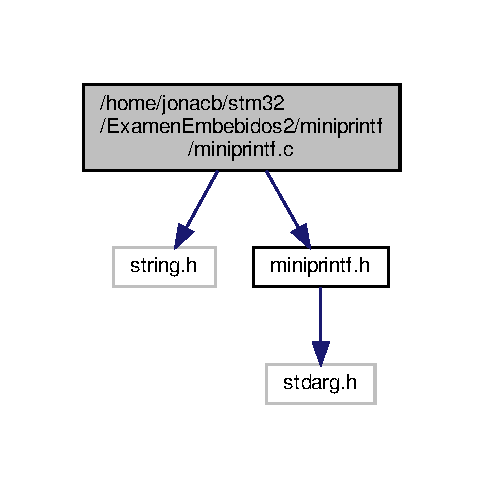
\includegraphics[width=232pt]{miniprintf_8c__incl}
\end{center}
\end{figure}
\subsection*{Classes}
\begin{DoxyCompactItemize}
\item 
struct \hyperlink{structs__mini__args}{s\+\_\+mini\+\_\+args}
\item 
struct \hyperlink{structs__internal}{s\+\_\+internal}
\item 
struct \hyperlink{structs__mini__sprintf}{s\+\_\+mini\+\_\+sprintf}
\end{DoxyCompactItemize}
\subsection*{Typedefs}
\begin{DoxyCompactItemize}
\item 
\mbox{\Hypertarget{miniprintf_8c_a77e49d83b074c279428b0cbb40dd26ec}\label{miniprintf_8c_a77e49d83b074c279428b0cbb40dd26ec}} 
typedef struct \hyperlink{structs__mini__args}{s\+\_\+mini\+\_\+args} {\bfseries miniarg\+\_\+t}
\end{DoxyCompactItemize}
\subsection*{Functions}
\begin{DoxyCompactItemize}
\item 
int \hyperlink{miniprintf_8c_a5bcf7f52ea6b2478c0ffb19d2ce4e5e5}{mini\+\_\+vprintf\+\_\+cooked} (void($\ast$putc)(char), const char $\ast$format, va\+\_\+list args)
\item 
int \hyperlink{miniprintf_8c_a1a532af594af9bb55f27718b227f5ccc}{mini\+\_\+vprintf\+\_\+uncooked} (void($\ast$putc)(char), const char $\ast$format, va\+\_\+list args)
\item 
int \hyperlink{miniprintf_8c_a9e466140f44967cb1b6310c5f57e2e86}{mini\+\_\+snprintf} (char $\ast$buf, unsigned maxbuf, const char $\ast$format,...)
\end{DoxyCompactItemize}


\subsection{Detailed Description}
miniprintf functions definitions. 



\subsection{Function Documentation}
\mbox{\Hypertarget{miniprintf_8c_a9e466140f44967cb1b6310c5f57e2e86}\label{miniprintf_8c_a9e466140f44967cb1b6310c5f57e2e86}} 
\index{miniprintf.\+c@{miniprintf.\+c}!mini\+\_\+snprintf@{mini\+\_\+snprintf}}
\index{mini\+\_\+snprintf@{mini\+\_\+snprintf}!miniprintf.\+c@{miniprintf.\+c}}
\subsubsection{\texorpdfstring{mini\+\_\+snprintf()}{mini\_snprintf()}}
{\footnotesize\ttfamily int mini\+\_\+snprintf (\begin{DoxyParamCaption}\item[{char $\ast$}]{buf,  }\item[{unsigned}]{maxbuf,  }\item[{const char $\ast$}]{format,  }\item[{}]{... }\end{DoxyParamCaption})}

External\+: sprintf() to buffer (not cooked) printf struct

sprintf control

format arguments

Return count

Internal routine

Using ctl to guide it

Destination for data

Max size in bytes

Calculate count

Null terminate output if possible

Return formatted count \mbox{\Hypertarget{miniprintf_8c_a5bcf7f52ea6b2478c0ffb19d2ce4e5e5}\label{miniprintf_8c_a5bcf7f52ea6b2478c0ffb19d2ce4e5e5}} 
\index{miniprintf.\+c@{miniprintf.\+c}!mini\+\_\+vprintf\+\_\+cooked@{mini\+\_\+vprintf\+\_\+cooked}}
\index{mini\+\_\+vprintf\+\_\+cooked@{mini\+\_\+vprintf\+\_\+cooked}!miniprintf.\+c@{miniprintf.\+c}}
\subsubsection{\texorpdfstring{mini\+\_\+vprintf\+\_\+cooked()}{mini\_vprintf\_cooked()}}
{\footnotesize\ttfamily int mini\+\_\+vprintf\+\_\+cooked (\begin{DoxyParamCaption}\item[{void($\ast$)(char)}]{putc,  }\item[{const char $\ast$}]{format,  }\item[{va\+\_\+list}]{args }\end{DoxyParamCaption})}

External\+: Perform cooked mode printf() \mbox{\Hypertarget{miniprintf_8c_a1a532af594af9bb55f27718b227f5ccc}\label{miniprintf_8c_a1a532af594af9bb55f27718b227f5ccc}} 
\index{miniprintf.\+c@{miniprintf.\+c}!mini\+\_\+vprintf\+\_\+uncooked@{mini\+\_\+vprintf\+\_\+uncooked}}
\index{mini\+\_\+vprintf\+\_\+uncooked@{mini\+\_\+vprintf\+\_\+uncooked}!miniprintf.\+c@{miniprintf.\+c}}
\subsubsection{\texorpdfstring{mini\+\_\+vprintf\+\_\+uncooked()}{mini\_vprintf\_uncooked()}}
{\footnotesize\ttfamily int mini\+\_\+vprintf\+\_\+uncooked (\begin{DoxyParamCaption}\item[{void($\ast$)(char)}]{putc,  }\item[{const char $\ast$}]{format,  }\item[{va\+\_\+list}]{args }\end{DoxyParamCaption})}

External\+: Perform uncooked (as is) printf() 
\hypertarget{miniprintf_8h}{}\section{/home/jonacb/stm32/\+Examen\+Embebidos2/miniprintf/miniprintf.h File Reference}
\label{miniprintf_8h}\index{/home/jonacb/stm32/\+Examen\+Embebidos2/miniprintf/miniprintf.\+h@{/home/jonacb/stm32/\+Examen\+Embebidos2/miniprintf/miniprintf.\+h}}


miniprintf header file.  


{\ttfamily \#include $<$stdarg.\+h$>$}\newline
Include dependency graph for miniprintf.\+h\+:\nopagebreak
\begin{figure}[H]
\begin{center}
\leavevmode
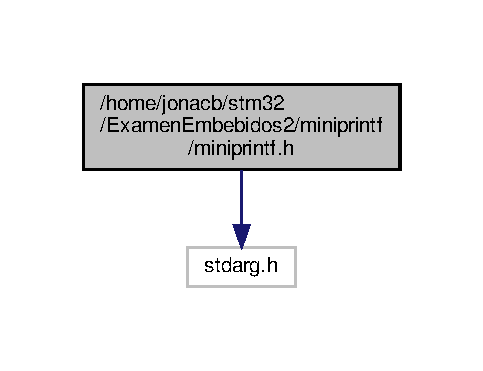
\includegraphics[width=232pt]{miniprintf_8h__incl}
\end{center}
\end{figure}
This graph shows which files directly or indirectly include this file\+:\nopagebreak
\begin{figure}[H]
\begin{center}
\leavevmode
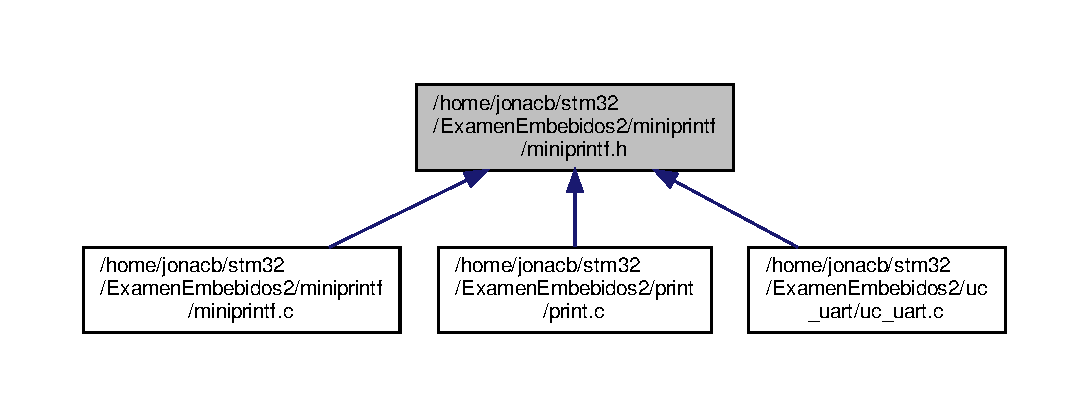
\includegraphics[width=350pt]{miniprintf_8h__dep__incl}
\end{center}
\end{figure}
\subsection*{Functions}
\begin{DoxyCompactItemize}
\item 
int \hyperlink{miniprintf_8h_a5bcf7f52ea6b2478c0ffb19d2ce4e5e5}{mini\+\_\+vprintf\+\_\+cooked} (void($\ast$putc)(char), const char $\ast$format, va\+\_\+list args)
\item 
int \hyperlink{miniprintf_8h_a1a532af594af9bb55f27718b227f5ccc}{mini\+\_\+vprintf\+\_\+uncooked} (void($\ast$putc)(char), const char $\ast$format, va\+\_\+list args)
\item 
\mbox{\Hypertarget{miniprintf_8h_aa3240298d52485708c33f9bc9afad641}\label{miniprintf_8h_aa3240298d52485708c33f9bc9afad641}} 
int {\bfseries mini\+\_\+snprintf} (char $\ast$buf, unsigned maxbuf, const char $\ast$format,...) \+\_\+\+\_\+attribute((format(printf
\end{DoxyCompactItemize}


\subsection{Detailed Description}
miniprintf header file. 



\subsection{Function Documentation}
\mbox{\Hypertarget{miniprintf_8h_a5bcf7f52ea6b2478c0ffb19d2ce4e5e5}\label{miniprintf_8h_a5bcf7f52ea6b2478c0ffb19d2ce4e5e5}} 
\index{miniprintf.\+h@{miniprintf.\+h}!mini\+\_\+vprintf\+\_\+cooked@{mini\+\_\+vprintf\+\_\+cooked}}
\index{mini\+\_\+vprintf\+\_\+cooked@{mini\+\_\+vprintf\+\_\+cooked}!miniprintf.\+h@{miniprintf.\+h}}
\subsubsection{\texorpdfstring{mini\+\_\+vprintf\+\_\+cooked()}{mini\_vprintf\_cooked()}}
{\footnotesize\ttfamily int mini\+\_\+vprintf\+\_\+cooked (\begin{DoxyParamCaption}\item[{void($\ast$)(char)}]{putc,  }\item[{const char $\ast$}]{format,  }\item[{va\+\_\+list}]{args }\end{DoxyParamCaption})}

External\+: Perform cooked mode printf() \mbox{\Hypertarget{miniprintf_8h_a1a532af594af9bb55f27718b227f5ccc}\label{miniprintf_8h_a1a532af594af9bb55f27718b227f5ccc}} 
\index{miniprintf.\+h@{miniprintf.\+h}!mini\+\_\+vprintf\+\_\+uncooked@{mini\+\_\+vprintf\+\_\+uncooked}}
\index{mini\+\_\+vprintf\+\_\+uncooked@{mini\+\_\+vprintf\+\_\+uncooked}!miniprintf.\+h@{miniprintf.\+h}}
\subsubsection{\texorpdfstring{mini\+\_\+vprintf\+\_\+uncooked()}{mini\_vprintf\_uncooked()}}
{\footnotesize\ttfamily int mini\+\_\+vprintf\+\_\+uncooked (\begin{DoxyParamCaption}\item[{void($\ast$)(char)}]{putc,  }\item[{const char $\ast$}]{format,  }\item[{va\+\_\+list}]{args }\end{DoxyParamCaption})}

External\+: Perform uncooked (as is) printf() 
\hypertarget{print_8c}{}\section{/home/jonacb/stm32/\+Examen\+Embebidos2/print/print.c File Reference}
\label{print_8c}\index{/home/jonacb/stm32/\+Examen\+Embebidos2/print/print.\+c@{/home/jonacb/stm32/\+Examen\+Embebidos2/print/print.\+c}}


Print functions definitions.  


{\ttfamily \#include \char`\"{}print.\+h\char`\"{}}\newline
{\ttfamily \#include \char`\"{}../uc\+\_\+uart/uc\+\_\+uart.\+h\char`\"{}}\newline
{\ttfamily \#include \char`\"{}../miniprintf/miniprintf.\+h\char`\"{}}\newline
Include dependency graph for print.\+c\+:\nopagebreak
\begin{figure}[H]
\begin{center}
\leavevmode
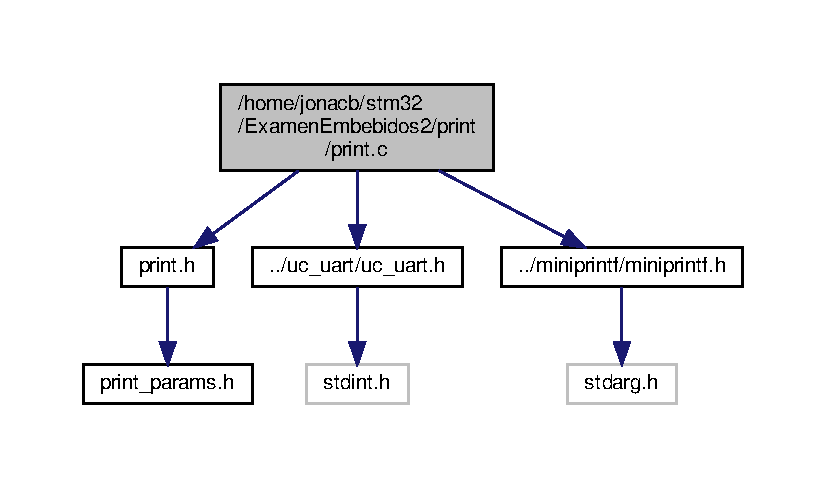
\includegraphics[width=350pt]{print_8c__incl}
\end{center}
\end{figure}
\subsection*{Functions}
\begin{DoxyCompactItemize}
\item 
void \hyperlink{print_8c_ab822ae4bef2935ed757393873841eb41}{print\+\_\+setup} (void)
\begin{DoxyCompactList}\small\item\em $<$Print header file. \end{DoxyCompactList}\item 
void \hyperlink{print_8c_a6483da854ca8076e0b947adaf1668954}{print} (const char $\ast$format,...)
\begin{DoxyCompactList}\small\item\em Function to print to console. \end{DoxyCompactList}\end{DoxyCompactItemize}


\subsection{Detailed Description}
Print functions definitions. 



\subsection{Function Documentation}
\mbox{\Hypertarget{print_8c_a6483da854ca8076e0b947adaf1668954}\label{print_8c_a6483da854ca8076e0b947adaf1668954}} 
\index{print.\+c@{print.\+c}!print@{print}}
\index{print@{print}!print.\+c@{print.\+c}}
\subsubsection{\texorpdfstring{print()}{print()}}
{\footnotesize\ttfamily void print (\begin{DoxyParamCaption}\item[{const char $\ast$}]{format,  }\item[{}]{... }\end{DoxyParamCaption})}



Function to print to console. 


\begin{DoxyParams}[1]{Parameters}
\mbox{\tt in}  & {\em format} & \\
\hline
\end{DoxyParams}
\mbox{\Hypertarget{print_8c_ab822ae4bef2935ed757393873841eb41}\label{print_8c_ab822ae4bef2935ed757393873841eb41}} 
\index{print.\+c@{print.\+c}!print\+\_\+setup@{print\+\_\+setup}}
\index{print\+\_\+setup@{print\+\_\+setup}!print.\+c@{print.\+c}}
\subsubsection{\texorpdfstring{print\+\_\+setup()}{print\_setup()}}
{\footnotesize\ttfamily void print\+\_\+setup (\begin{DoxyParamCaption}\item[{void}]{ }\end{DoxyParamCaption})}



$<$Print header file. 

$<$Include print parameters.

$<$Miniprint include. Sets up parameters needed to print to console. 
\hypertarget{print_8h}{}\section{/home/jonacb/stm32/\+Examen\+Embebidos2/print/print.h File Reference}
\label{print_8h}\index{/home/jonacb/stm32/\+Examen\+Embebidos2/print/print.\+h@{/home/jonacb/stm32/\+Examen\+Embebidos2/print/print.\+h}}


Print function headers.  


{\ttfamily \#include \char`\"{}print\+\_\+params.\+h\char`\"{}}\newline
Include dependency graph for print.\+h\+:\nopagebreak
\begin{figure}[H]
\begin{center}
\leavevmode
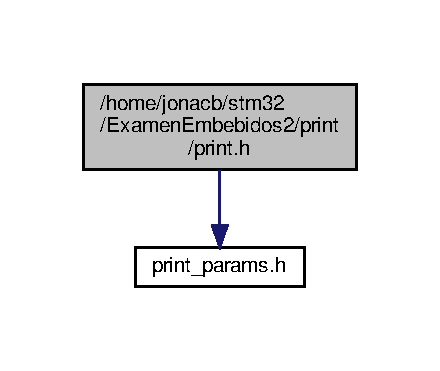
\includegraphics[width=211pt]{print_8h__incl}
\end{center}
\end{figure}
This graph shows which files directly or indirectly include this file\+:\nopagebreak
\begin{figure}[H]
\begin{center}
\leavevmode
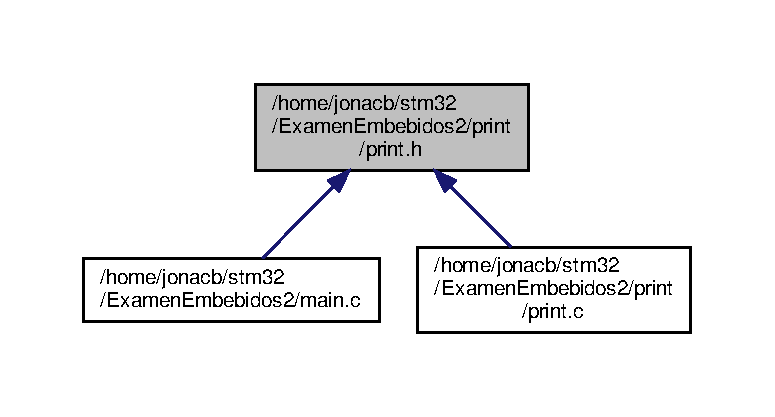
\includegraphics[width=350pt]{print_8h__dep__incl}
\end{center}
\end{figure}
\subsection*{Functions}
\begin{DoxyCompactItemize}
\item 
void \hyperlink{print_8h_ab822ae4bef2935ed757393873841eb41}{print\+\_\+setup} (void)
\begin{DoxyCompactList}\small\item\em $<$Include print parameters. \end{DoxyCompactList}\item 
void \hyperlink{print_8h_a6483da854ca8076e0b947adaf1668954}{print} (const char $\ast$format,...)
\begin{DoxyCompactList}\small\item\em Function to print to console. \end{DoxyCompactList}\end{DoxyCompactItemize}


\subsection{Detailed Description}
Print function headers. 



\subsection{Function Documentation}
\mbox{\Hypertarget{print_8h_a6483da854ca8076e0b947adaf1668954}\label{print_8h_a6483da854ca8076e0b947adaf1668954}} 
\index{print.\+h@{print.\+h}!print@{print}}
\index{print@{print}!print.\+h@{print.\+h}}
\subsubsection{\texorpdfstring{print()}{print()}}
{\footnotesize\ttfamily void print (\begin{DoxyParamCaption}\item[{const char $\ast$}]{format,  }\item[{}]{... }\end{DoxyParamCaption})}



Function to print to console. 


\begin{DoxyParams}[1]{Parameters}
\mbox{\tt in}  & {\em format} & \\
\hline
\end{DoxyParams}
\mbox{\Hypertarget{print_8h_ab822ae4bef2935ed757393873841eb41}\label{print_8h_ab822ae4bef2935ed757393873841eb41}} 
\index{print.\+h@{print.\+h}!print\+\_\+setup@{print\+\_\+setup}}
\index{print\+\_\+setup@{print\+\_\+setup}!print.\+h@{print.\+h}}
\subsubsection{\texorpdfstring{print\+\_\+setup()}{print\_setup()}}
{\footnotesize\ttfamily void print\+\_\+setup (\begin{DoxyParamCaption}\item[{void}]{ }\end{DoxyParamCaption})}



$<$Include print parameters. 

$<$Include print parameters.

$<$Miniprint include. Sets up parameters needed to print to console. 
\hypertarget{print__params_8h}{}\section{/home/jonacb/stm32/\+Examen\+Embebidos2/print/print\+\_\+params.h File Reference}
\label{print__params_8h}\index{/home/jonacb/stm32/\+Examen\+Embebidos2/print/print\+\_\+params.\+h@{/home/jonacb/stm32/\+Examen\+Embebidos2/print/print\+\_\+params.\+h}}


Definition of parameters used to configure the U\+A\+RT.  


This graph shows which files directly or indirectly include this file\+:\nopagebreak
\begin{figure}[H]
\begin{center}
\leavevmode
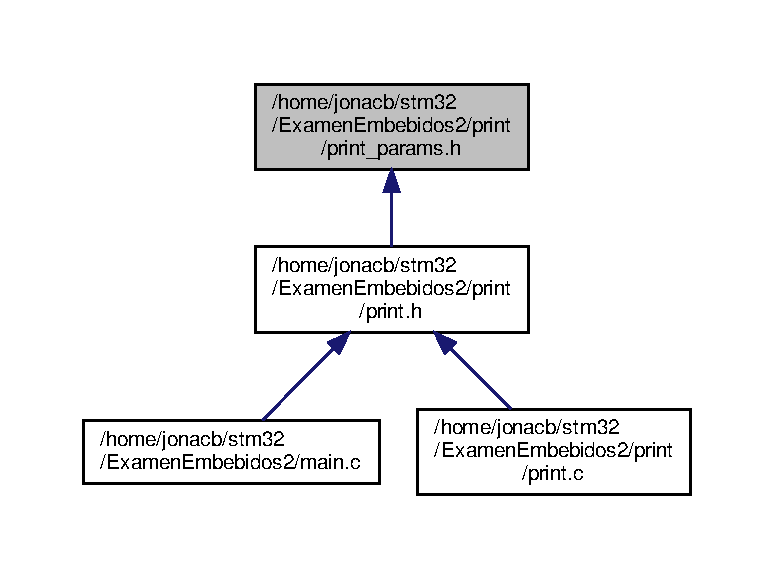
\includegraphics[width=350pt]{print__params_8h__dep__incl}
\end{center}
\end{figure}
\subsection*{Macros}
\begin{DoxyCompactItemize}
\item 
\mbox{\Hypertarget{print__params_8h_a8b2ea1898f38cfe1f20ca4e2e155e2bd}\label{print__params_8h_a8b2ea1898f38cfe1f20ca4e2e155e2bd}} 
\#define \hyperlink{print__params_8h_a8b2ea1898f38cfe1f20ca4e2e155e2bd}{U\+A\+R\+T\+\_\+\+T\+X\+\_\+\+P\+O\+RT}~1
\begin{DoxyCompactList}\small\item\em U\+A\+RT Transmitter port used. \end{DoxyCompactList}\item 
\mbox{\Hypertarget{print__params_8h_a6c82a6844388a551e8f06d249598989e}\label{print__params_8h_a6c82a6844388a551e8f06d249598989e}} 
\#define \hyperlink{print__params_8h_a6c82a6844388a551e8f06d249598989e}{U\+A\+R\+T\+\_\+\+T\+X\+\_\+\+P\+IN}~1
\begin{DoxyCompactList}\small\item\em U\+A\+RT Transmitter pin used. \end{DoxyCompactList}\item 
\mbox{\Hypertarget{print__params_8h_a151b6aa11aa5aad16c7468122af3b3a3}\label{print__params_8h_a151b6aa11aa5aad16c7468122af3b3a3}} 
\#define \hyperlink{print__params_8h_a151b6aa11aa5aad16c7468122af3b3a3}{U\+A\+R\+T\+\_\+\+R\+X\+\_\+\+P\+O\+RT}~1
\begin{DoxyCompactList}\small\item\em U\+A\+RT Receiver port used. \end{DoxyCompactList}\item 
\mbox{\Hypertarget{print__params_8h_aa37eca6fe61f6938d925975dff27c8fd}\label{print__params_8h_aa37eca6fe61f6938d925975dff27c8fd}} 
\#define \hyperlink{print__params_8h_aa37eca6fe61f6938d925975dff27c8fd}{U\+A\+R\+T\+\_\+\+R\+X\+\_\+\+P\+IN}~1
\begin{DoxyCompactList}\small\item\em U\+A\+RT Receiver pin used. \end{DoxyCompactList}\item 
\mbox{\Hypertarget{print__params_8h_af7cb12b462b4594bd759d1b4e241ec4c}\label{print__params_8h_af7cb12b462b4594bd759d1b4e241ec4c}} 
\#define \hyperlink{print__params_8h_af7cb12b462b4594bd759d1b4e241ec4c}{U\+A\+RT}~1
\begin{DoxyCompactList}\small\item\em U\+A\+RT to be used. \end{DoxyCompactList}\item 
\mbox{\Hypertarget{print__params_8h_a734bbab06e1a9fd2e5522db0221ff6e3}\label{print__params_8h_a734bbab06e1a9fd2e5522db0221ff6e3}} 
\#define \hyperlink{print__params_8h_a734bbab06e1a9fd2e5522db0221ff6e3}{B\+A\+U\+D\+R\+A\+TE}~115200
\begin{DoxyCompactList}\small\item\em U\+A\+RT baudrate configuration. \end{DoxyCompactList}\item 
\mbox{\Hypertarget{print__params_8h_a155a9a6160c909e29d95e7c75b79612a}\label{print__params_8h_a155a9a6160c909e29d95e7c75b79612a}} 
\#define \hyperlink{print__params_8h_a155a9a6160c909e29d95e7c75b79612a}{D\+A\+T\+A\+B\+I\+TS}~8
\begin{DoxyCompactList}\small\item\em U\+A\+RT data width configuration. \end{DoxyCompactList}\end{DoxyCompactItemize}


\subsection{Detailed Description}
Definition of parameters used to configure the U\+A\+RT. 


\hypertarget{system__common_8c}{}\section{/home/jonacb/stm32/\+Examen\+Embebidos2/system\+\_\+common/system\+\_\+common.c File Reference}
\label{system__common_8c}\index{/home/jonacb/stm32/\+Examen\+Embebidos2/system\+\_\+common/system\+\_\+common.\+c@{/home/jonacb/stm32/\+Examen\+Embebidos2/system\+\_\+common/system\+\_\+common.\+c}}
{\ttfamily \#include \char`\"{}system\+\_\+common.\+h\char`\"{}}\newline
Include dependency graph for system\+\_\+common.\+c\+:\nopagebreak
\begin{figure}[H]
\begin{center}
\leavevmode
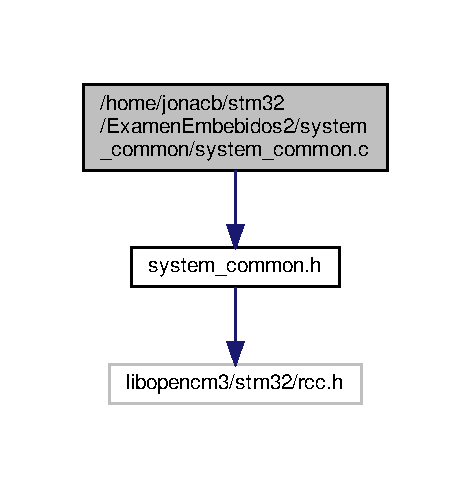
\includegraphics[width=226pt]{system__common_8c__incl}
\end{center}
\end{figure}
\subsection*{Functions}
\begin{DoxyCompactItemize}
\item 
void \hyperlink{system__common_8c_aceb396639c7aff9aba7440f22465f59a}{system\+\_\+clock\+\_\+setup} (void)
\end{DoxyCompactItemize}


\subsection{Function Documentation}
\mbox{\Hypertarget{system__common_8c_aceb396639c7aff9aba7440f22465f59a}\label{system__common_8c_aceb396639c7aff9aba7440f22465f59a}} 
\index{system\+\_\+common.\+c@{system\+\_\+common.\+c}!system\+\_\+clock\+\_\+setup@{system\+\_\+clock\+\_\+setup}}
\index{system\+\_\+clock\+\_\+setup@{system\+\_\+clock\+\_\+setup}!system\+\_\+common.\+c@{system\+\_\+common.\+c}}
\subsubsection{\texorpdfstring{system\+\_\+clock\+\_\+setup()}{system\_clock\_setup()}}
{\footnotesize\ttfamily void system\+\_\+clock\+\_\+setup (\begin{DoxyParamCaption}\item[{void}]{ }\end{DoxyParamCaption})}

Sets up the system clock frequency. 
\hypertarget{system__common_8h}{}\section{/home/jonacb/stm32/\+Examen\+Embebidos2/system\+\_\+common/system\+\_\+common.h File Reference}
\label{system__common_8h}\index{/home/jonacb/stm32/\+Examen\+Embebidos2/system\+\_\+common/system\+\_\+common.\+h@{/home/jonacb/stm32/\+Examen\+Embebidos2/system\+\_\+common/system\+\_\+common.\+h}}


system\+\_\+common header file.  


{\ttfamily \#include $<$libopencm3/stm32/rcc.\+h$>$}\newline
Include dependency graph for system\+\_\+common.\+h\+:\nopagebreak
\begin{figure}[H]
\begin{center}
\leavevmode
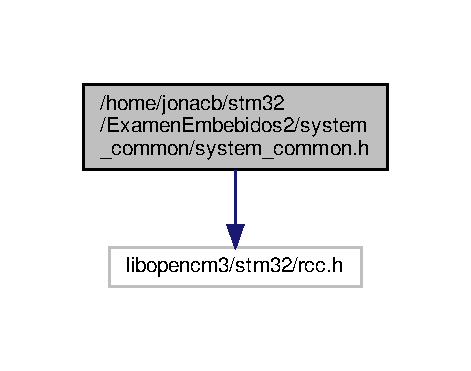
\includegraphics[width=226pt]{system__common_8h__incl}
\end{center}
\end{figure}
This graph shows which files directly or indirectly include this file\+:\nopagebreak
\begin{figure}[H]
\begin{center}
\leavevmode
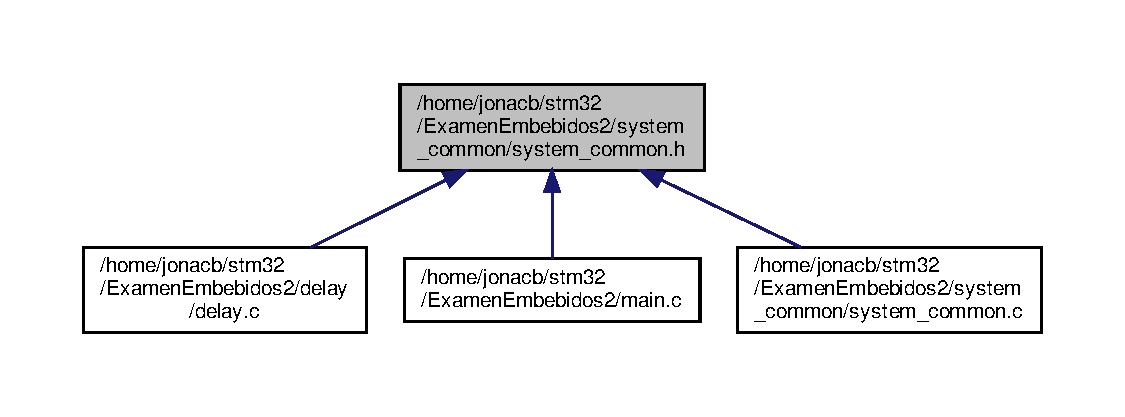
\includegraphics[width=350pt]{system__common_8h__dep__incl}
\end{center}
\end{figure}
\subsection*{Macros}
\begin{DoxyCompactItemize}
\item 
\mbox{\Hypertarget{system__common_8h_a2368e20d446b5abc7e62f36b9b66e07c}\label{system__common_8h_a2368e20d446b5abc7e62f36b9b66e07c}} 
\#define \hyperlink{system__common_8h_a2368e20d446b5abc7e62f36b9b66e07c}{F\+\_\+\+C\+LK}~72000000
\begin{DoxyCompactList}\small\item\em Clock constant define. \end{DoxyCompactList}\end{DoxyCompactItemize}
\subsection*{Functions}
\begin{DoxyCompactItemize}
\item 
void \hyperlink{system__common_8h_aceb396639c7aff9aba7440f22465f59a}{system\+\_\+clock\+\_\+setup} (void)
\end{DoxyCompactItemize}


\subsection{Detailed Description}
system\+\_\+common header file. 



\subsection{Function Documentation}
\mbox{\Hypertarget{system__common_8h_aceb396639c7aff9aba7440f22465f59a}\label{system__common_8h_aceb396639c7aff9aba7440f22465f59a}} 
\index{system\+\_\+common.\+h@{system\+\_\+common.\+h}!system\+\_\+clock\+\_\+setup@{system\+\_\+clock\+\_\+setup}}
\index{system\+\_\+clock\+\_\+setup@{system\+\_\+clock\+\_\+setup}!system\+\_\+common.\+h@{system\+\_\+common.\+h}}
\subsubsection{\texorpdfstring{system\+\_\+clock\+\_\+setup()}{system\_clock\_setup()}}
{\footnotesize\ttfamily void system\+\_\+clock\+\_\+setup (\begin{DoxyParamCaption}\item[{void}]{ }\end{DoxyParamCaption})}

Sets up the system clock frequency. 
\hypertarget{timer_8c}{}\section{/home/jonacb/stm32/\+Examen\+Embebidos2/timer/timer.c File Reference}
\label{timer_8c}\index{/home/jonacb/stm32/\+Examen\+Embebidos2/timer/timer.\+c@{/home/jonacb/stm32/\+Examen\+Embebidos2/timer/timer.\+c}}


Timer functions definition.  


{\ttfamily \#include \char`\"{}timer.\+h\char`\"{}}\newline
{\ttfamily \#include \char`\"{}../uc\+\_\+timer/uc\+\_\+timer.\+h\char`\"{}}\newline
Include dependency graph for timer.\+c\+:\nopagebreak
\begin{figure}[H]
\begin{center}
\leavevmode
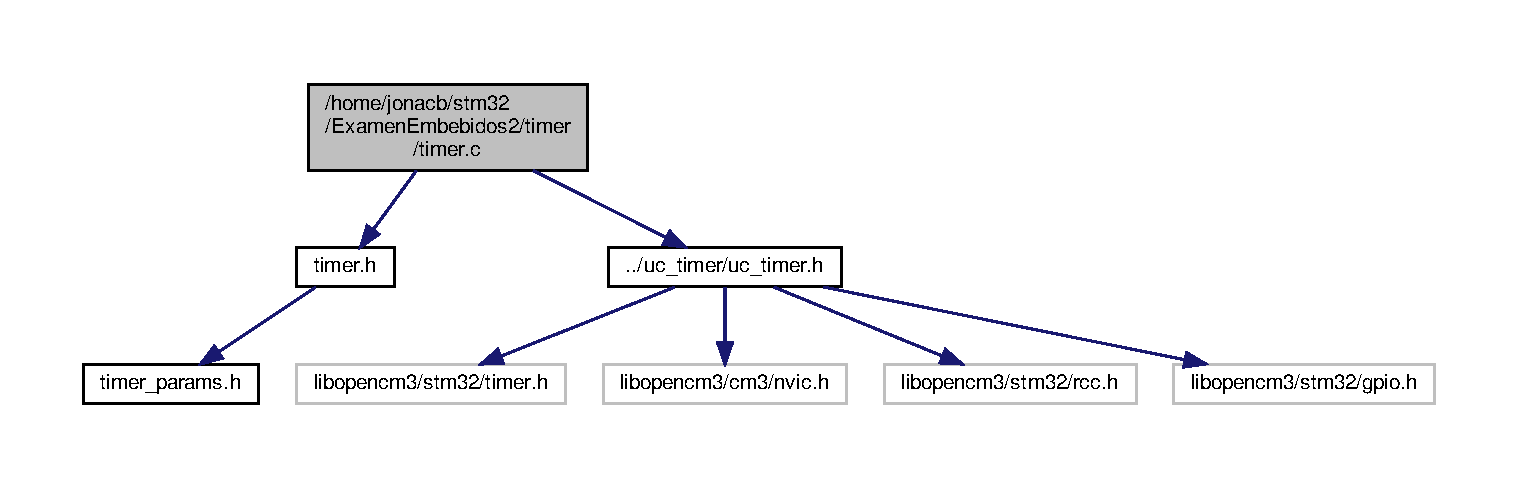
\includegraphics[width=350pt]{timer_8c__incl}
\end{center}
\end{figure}
\subsection*{Functions}
\begin{DoxyCompactItemize}
\item 
void \hyperlink{timer_8c_aa3fa978d501dc3291b65edd419727976}{timer\+\_\+setup} (void)
\begin{DoxyCompactList}\small\item\em $<$Timer header file. \end{DoxyCompactList}\item 
\mbox{\Hypertarget{timer_8c_a51b21406d70a1c23098b39be29dd0ffb}\label{timer_8c_a51b21406d70a1c23098b39be29dd0ffb}} 
void \hyperlink{timer_8c_a51b21406d70a1c23098b39be29dd0ffb}{timer\+\_\+rst} (void)
\begin{DoxyCompactList}\small\item\em Resets the timer. \end{DoxyCompactList}\item 
\mbox{\Hypertarget{timer_8c_aeb09db6f93d0e0f5aad6e9d2345793e0}\label{timer_8c_aeb09db6f93d0e0f5aad6e9d2345793e0}} 
void \hyperlink{timer_8c_aeb09db6f93d0e0f5aad6e9d2345793e0}{timer\+\_\+start} (void)
\begin{DoxyCompactList}\small\item\em Starts the timer. \end{DoxyCompactList}\item 
\mbox{\Hypertarget{timer_8c_a37980fc313f86d7f40a3d7643861ed29}\label{timer_8c_a37980fc313f86d7f40a3d7643861ed29}} 
void \hyperlink{timer_8c_a37980fc313f86d7f40a3d7643861ed29}{timer\+\_\+stop} (void)
\begin{DoxyCompactList}\small\item\em Pauses the timer. \end{DoxyCompactList}\item 
\mbox{\Hypertarget{timer_8c_a1b6d6adead99166fecc0c496d80d7415}\label{timer_8c_a1b6d6adead99166fecc0c496d80d7415}} 
void \hyperlink{timer_8c_a1b6d6adead99166fecc0c496d80d7415}{timer\+\_\+continue} (void)
\begin{DoxyCompactList}\small\item\em Unpauses the timer. \end{DoxyCompactList}\item 
int \hyperlink{timer_8c_ac8a45dbca33f3059dbaa78add301f01d}{timer\+\_\+get\+\_\+seconds} (void)
\begin{DoxyCompactList}\small\item\em Returns the counts of the timer in seconds. \end{DoxyCompactList}\end{DoxyCompactItemize}


\subsection{Detailed Description}
Timer functions definition. 



\subsection{Function Documentation}
\mbox{\Hypertarget{timer_8c_ac8a45dbca33f3059dbaa78add301f01d}\label{timer_8c_ac8a45dbca33f3059dbaa78add301f01d}} 
\index{timer.\+c@{timer.\+c}!timer\+\_\+get\+\_\+seconds@{timer\+\_\+get\+\_\+seconds}}
\index{timer\+\_\+get\+\_\+seconds@{timer\+\_\+get\+\_\+seconds}!timer.\+c@{timer.\+c}}
\subsubsection{\texorpdfstring{timer\+\_\+get\+\_\+seconds()}{timer\_get\_seconds()}}
{\footnotesize\ttfamily int timer\+\_\+get\+\_\+seconds (\begin{DoxyParamCaption}\item[{void}]{ }\end{DoxyParamCaption})}



Returns the counts of the timer in seconds. 

\begin{DoxyReturn}{Returns}
timer\+\_\+count 
\end{DoxyReturn}
\mbox{\Hypertarget{timer_8c_aa3fa978d501dc3291b65edd419727976}\label{timer_8c_aa3fa978d501dc3291b65edd419727976}} 
\index{timer.\+c@{timer.\+c}!timer\+\_\+setup@{timer\+\_\+setup}}
\index{timer\+\_\+setup@{timer\+\_\+setup}!timer.\+c@{timer.\+c}}
\subsubsection{\texorpdfstring{timer\+\_\+setup()}{timer\_setup()}}
{\footnotesize\ttfamily void timer\+\_\+setup (\begin{DoxyParamCaption}\item[{void}]{ }\end{DoxyParamCaption})}



$<$Timer header file. 

$<$T\+I\+M\+ER params header include.

Sets up the timer. 
\hypertarget{timer_8h}{}\section{/home/jonacb/stm32/\+Examen\+Embebidos2/timer/timer.h File Reference}
\label{timer_8h}\index{/home/jonacb/stm32/\+Examen\+Embebidos2/timer/timer.\+h@{/home/jonacb/stm32/\+Examen\+Embebidos2/timer/timer.\+h}}


T\+I\+M\+ER header file.  


{\ttfamily \#include \char`\"{}timer\+\_\+params.\+h\char`\"{}}\newline
Include dependency graph for timer.\+h\+:\nopagebreak
\begin{figure}[H]
\begin{center}
\leavevmode
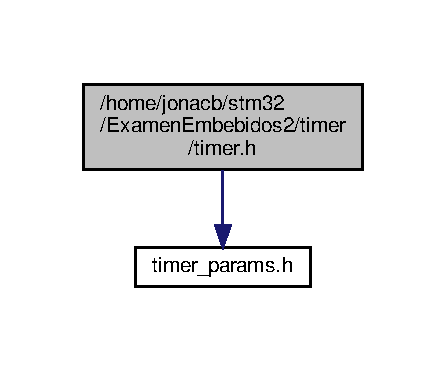
\includegraphics[width=214pt]{timer_8h__incl}
\end{center}
\end{figure}
This graph shows which files directly or indirectly include this file\+:\nopagebreak
\begin{figure}[H]
\begin{center}
\leavevmode
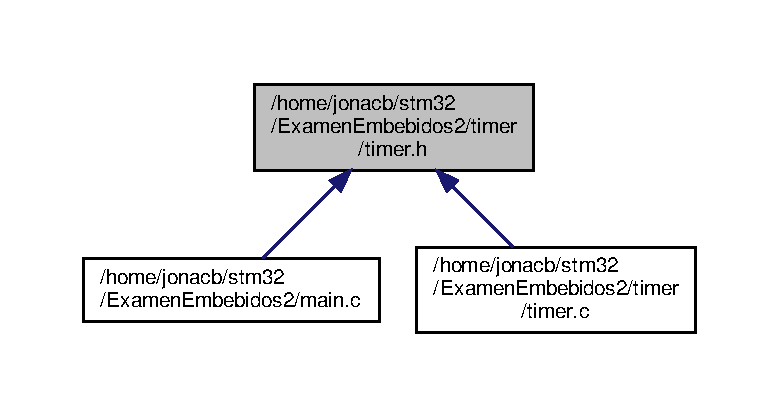
\includegraphics[width=350pt]{timer_8h__dep__incl}
\end{center}
\end{figure}
\subsection*{Functions}
\begin{DoxyCompactItemize}
\item 
void \hyperlink{timer_8h_aa3fa978d501dc3291b65edd419727976}{timer\+\_\+setup} (void)
\begin{DoxyCompactList}\small\item\em $<$T\+I\+M\+ER params header include. \end{DoxyCompactList}\item 
\mbox{\Hypertarget{timer_8h_a51b21406d70a1c23098b39be29dd0ffb}\label{timer_8h_a51b21406d70a1c23098b39be29dd0ffb}} 
void \hyperlink{timer_8h_a51b21406d70a1c23098b39be29dd0ffb}{timer\+\_\+rst} (void)
\begin{DoxyCompactList}\small\item\em Resets the timer. \end{DoxyCompactList}\item 
\mbox{\Hypertarget{timer_8h_aeb09db6f93d0e0f5aad6e9d2345793e0}\label{timer_8h_aeb09db6f93d0e0f5aad6e9d2345793e0}} 
void \hyperlink{timer_8h_aeb09db6f93d0e0f5aad6e9d2345793e0}{timer\+\_\+start} (void)
\begin{DoxyCompactList}\small\item\em Starts the timer. \end{DoxyCompactList}\item 
\mbox{\Hypertarget{timer_8h_a37980fc313f86d7f40a3d7643861ed29}\label{timer_8h_a37980fc313f86d7f40a3d7643861ed29}} 
void \hyperlink{timer_8h_a37980fc313f86d7f40a3d7643861ed29}{timer\+\_\+stop} (void)
\begin{DoxyCompactList}\small\item\em Pauses the timer. \end{DoxyCompactList}\item 
\mbox{\Hypertarget{timer_8h_a1b6d6adead99166fecc0c496d80d7415}\label{timer_8h_a1b6d6adead99166fecc0c496d80d7415}} 
void \hyperlink{timer_8h_a1b6d6adead99166fecc0c496d80d7415}{timer\+\_\+continue} (void)
\begin{DoxyCompactList}\small\item\em Unpauses the timer. \end{DoxyCompactList}\item 
int \hyperlink{timer_8h_ac8a45dbca33f3059dbaa78add301f01d}{timer\+\_\+get\+\_\+seconds} (void)
\begin{DoxyCompactList}\small\item\em Returns the counts of the timer in seconds. \end{DoxyCompactList}\end{DoxyCompactItemize}


\subsection{Detailed Description}
T\+I\+M\+ER header file. 



\subsection{Function Documentation}
\mbox{\Hypertarget{timer_8h_ac8a45dbca33f3059dbaa78add301f01d}\label{timer_8h_ac8a45dbca33f3059dbaa78add301f01d}} 
\index{timer.\+h@{timer.\+h}!timer\+\_\+get\+\_\+seconds@{timer\+\_\+get\+\_\+seconds}}
\index{timer\+\_\+get\+\_\+seconds@{timer\+\_\+get\+\_\+seconds}!timer.\+h@{timer.\+h}}
\subsubsection{\texorpdfstring{timer\+\_\+get\+\_\+seconds()}{timer\_get\_seconds()}}
{\footnotesize\ttfamily int timer\+\_\+get\+\_\+seconds (\begin{DoxyParamCaption}\item[{void}]{ }\end{DoxyParamCaption})}



Returns the counts of the timer in seconds. 

\begin{DoxyReturn}{Returns}
timer\+\_\+count 
\end{DoxyReturn}
\mbox{\Hypertarget{timer_8h_aa3fa978d501dc3291b65edd419727976}\label{timer_8h_aa3fa978d501dc3291b65edd419727976}} 
\index{timer.\+h@{timer.\+h}!timer\+\_\+setup@{timer\+\_\+setup}}
\index{timer\+\_\+setup@{timer\+\_\+setup}!timer.\+h@{timer.\+h}}
\subsubsection{\texorpdfstring{timer\+\_\+setup()}{timer\_setup()}}
{\footnotesize\ttfamily void timer\+\_\+setup (\begin{DoxyParamCaption}\item[{void}]{ }\end{DoxyParamCaption})}



$<$T\+I\+M\+ER params header include. 

$<$T\+I\+M\+ER params header include.

Sets up the timer. 
\hypertarget{uc__timer_8c}{}\doxysection{Git\+Hub/\+Sistemas\+Embebidos\+Tec\+G\+D\+A/\+Abstraction\+\_\+and\+\_\+documentation/uc\+\_\+timer/uc\+\_\+timer.c File Reference}
\label{uc__timer_8c}\index{GitHub/SistemasEmbebidosTecGDA/Abstraction\_and\_documentation/uc\_timer/uc\_timer.c@{GitHub/SistemasEmbebidosTecGDA/Abstraction\_and\_documentation/uc\_timer/uc\_timer.c}}
{\ttfamily \#include \char`\"{}uc\+\_\+timer.\+h\char`\"{}}\newline
\doxysubsection*{Functions}
\begin{DoxyCompactItemize}
\item 
void \mbox{\hyperlink{uc__timer_8c_a58293981ed0469d0d2b0cc0e70beecce}{uc\+\_\+timer\+\_\+pwm\+\_\+pin\+\_\+setup}} (enum rcc\+\_\+periph\+\_\+clken gpio\+\_\+clk, uint32\+\_\+t gpio\+\_\+port, uint16\+\_\+t gpio\+\_\+pin)
\item 
void \mbox{\hyperlink{uc__timer_8c_aa32fe1c6f887bf184010424db5634198}{uc\+\_\+timer\+\_\+setup}} (enum rcc\+\_\+periph\+\_\+clken timer\+\_\+clk, uint32\+\_\+t timer, uint32\+\_\+t prescaler)
\item 
void \mbox{\hyperlink{uc__timer_8c_a3783dcda7914f2a5113a276bbb6d886d}{uc\+\_\+timer\+\_\+pwm\+\_\+setup}} (enum rcc\+\_\+periph\+\_\+clken timer\+\_\+clk, uint32\+\_\+t timer, enum tim\+\_\+oc\+\_\+id channel, uint32\+\_\+t prescaler)
\item 
void \mbox{\hyperlink{uc__timer_8c_a5ace3c51af58c627a2448d7af70f170f}{uc\+\_\+timer\+\_\+config\+\_\+period}} (uint32\+\_\+t timer, uint32\+\_\+t period)
\item 
void \mbox{\hyperlink{uc__timer_8c_a1ca803f1f79b91d0fa7622bf5161b94e}{uc\+\_\+timer\+\_\+pwm\+\_\+config\+\_\+duty\+\_\+cycle}} (uint32\+\_\+t timer, enum tim\+\_\+oc\+\_\+id channel, uint32\+\_\+t duty\+\_\+cycle)
\item 
void \mbox{\hyperlink{uc__timer_8c_ac1f3c225897cfdee7111bcf69ffd0222}{uc\+\_\+timer\+\_\+enable\+\_\+interrupt}} (uint32\+\_\+t timer, uint8\+\_\+t irqn)
\item 
void \mbox{\hyperlink{uc__timer_8c_a4962fd7b57586816079db0aa487091d3}{uc\+\_\+timer\+\_\+start}} (uint32\+\_\+t timer)
\item 
void \mbox{\hyperlink{uc__timer_8c_ab7c0468c8d4fc8bf514ada5ee90671e5}{uc\+\_\+timer\+\_\+stop}} (uint32\+\_\+t timer)
\end{DoxyCompactItemize}


\doxysubsection{Function Documentation}
\mbox{\Hypertarget{uc__timer_8c_a5ace3c51af58c627a2448d7af70f170f}\label{uc__timer_8c_a5ace3c51af58c627a2448d7af70f170f}} 
\index{uc\_timer.c@{uc\_timer.c}!uc\_timer\_config\_period@{uc\_timer\_config\_period}}
\index{uc\_timer\_config\_period@{uc\_timer\_config\_period}!uc\_timer.c@{uc\_timer.c}}
\doxysubsubsection{\texorpdfstring{uc\_timer\_config\_period()}{uc\_timer\_config\_period()}}
{\footnotesize\ttfamily void uc\+\_\+timer\+\_\+config\+\_\+period (\begin{DoxyParamCaption}\item[{uint32\+\_\+t}]{timer,  }\item[{uint32\+\_\+t}]{period }\end{DoxyParamCaption})}

Configures the timer\textquotesingle{}s period. 
\begin{DoxyParams}[1]{Parameters}
\mbox{\texttt{ in}}  & {\em timer} & \\
\hline
\mbox{\texttt{ in}}  & {\em period} & \\
\hline
\end{DoxyParams}
\mbox{\Hypertarget{uc__timer_8c_ac1f3c225897cfdee7111bcf69ffd0222}\label{uc__timer_8c_ac1f3c225897cfdee7111bcf69ffd0222}} 
\index{uc\_timer.c@{uc\_timer.c}!uc\_timer\_enable\_interrupt@{uc\_timer\_enable\_interrupt}}
\index{uc\_timer\_enable\_interrupt@{uc\_timer\_enable\_interrupt}!uc\_timer.c@{uc\_timer.c}}
\doxysubsubsection{\texorpdfstring{uc\_timer\_enable\_interrupt()}{uc\_timer\_enable\_interrupt()}}
{\footnotesize\ttfamily void uc\+\_\+timer\+\_\+enable\+\_\+interrupt (\begin{DoxyParamCaption}\item[{uint32\+\_\+t}]{timer,  }\item[{uint8\+\_\+t}]{irqn }\end{DoxyParamCaption})}

Enables timer\textquotesingle{}s interrupt. 
\begin{DoxyParams}[1]{Parameters}
\mbox{\texttt{ in}}  & {\em timer} & \\
\hline
\mbox{\texttt{ in}}  & {\em irqn} & \\
\hline
\end{DoxyParams}
\mbox{\Hypertarget{uc__timer_8c_a1ca803f1f79b91d0fa7622bf5161b94e}\label{uc__timer_8c_a1ca803f1f79b91d0fa7622bf5161b94e}} 
\index{uc\_timer.c@{uc\_timer.c}!uc\_timer\_pwm\_config\_duty\_cycle@{uc\_timer\_pwm\_config\_duty\_cycle}}
\index{uc\_timer\_pwm\_config\_duty\_cycle@{uc\_timer\_pwm\_config\_duty\_cycle}!uc\_timer.c@{uc\_timer.c}}
\doxysubsubsection{\texorpdfstring{uc\_timer\_pwm\_config\_duty\_cycle()}{uc\_timer\_pwm\_config\_duty\_cycle()}}
{\footnotesize\ttfamily void uc\+\_\+timer\+\_\+pwm\+\_\+config\+\_\+duty\+\_\+cycle (\begin{DoxyParamCaption}\item[{uint32\+\_\+t}]{timer,  }\item[{enum tim\+\_\+oc\+\_\+id}]{channel,  }\item[{uint32\+\_\+t}]{duty\+\_\+cycle }\end{DoxyParamCaption})}

Configures the timer\textquotesingle{}s pwm duty cycle. 
\begin{DoxyParams}[1]{Parameters}
\mbox{\texttt{ in}}  & {\em timer} & \\
\hline
\mbox{\texttt{ in}}  & {\em channel} & \\
\hline
\end{DoxyParams}
\mbox{\Hypertarget{uc__timer_8c_a58293981ed0469d0d2b0cc0e70beecce}\label{uc__timer_8c_a58293981ed0469d0d2b0cc0e70beecce}} 
\index{uc\_timer.c@{uc\_timer.c}!uc\_timer\_pwm\_pin\_setup@{uc\_timer\_pwm\_pin\_setup}}
\index{uc\_timer\_pwm\_pin\_setup@{uc\_timer\_pwm\_pin\_setup}!uc\_timer.c@{uc\_timer.c}}
\doxysubsubsection{\texorpdfstring{uc\_timer\_pwm\_pin\_setup()}{uc\_timer\_pwm\_pin\_setup()}}
{\footnotesize\ttfamily void uc\+\_\+timer\+\_\+pwm\+\_\+pin\+\_\+setup (\begin{DoxyParamCaption}\item[{enum rcc\+\_\+periph\+\_\+clken}]{gpio\+\_\+clk,  }\item[{uint32\+\_\+t}]{gpio\+\_\+port,  }\item[{uint16\+\_\+t}]{gpio\+\_\+pin }\end{DoxyParamCaption})}

Sets up the P\+WM peripheral pin ports needed. 
\begin{DoxyParams}[1]{Parameters}
\mbox{\texttt{ in}}  & {\em gpio\+\_\+clk} & \\
\hline
\mbox{\texttt{ in}}  & {\em gpio\+\_\+port} & \\
\hline
\mbox{\texttt{ in}}  & {\em gpio\+\_\+pin} & \\
\hline
\end{DoxyParams}
\mbox{\Hypertarget{uc__timer_8c_a3783dcda7914f2a5113a276bbb6d886d}\label{uc__timer_8c_a3783dcda7914f2a5113a276bbb6d886d}} 
\index{uc\_timer.c@{uc\_timer.c}!uc\_timer\_pwm\_setup@{uc\_timer\_pwm\_setup}}
\index{uc\_timer\_pwm\_setup@{uc\_timer\_pwm\_setup}!uc\_timer.c@{uc\_timer.c}}
\doxysubsubsection{\texorpdfstring{uc\_timer\_pwm\_setup()}{uc\_timer\_pwm\_setup()}}
{\footnotesize\ttfamily void uc\+\_\+timer\+\_\+pwm\+\_\+setup (\begin{DoxyParamCaption}\item[{enum rcc\+\_\+periph\+\_\+clken}]{timer\+\_\+clk,  }\item[{uint32\+\_\+t}]{timer,  }\item[{enum tim\+\_\+oc\+\_\+id}]{channel,  }\item[{uint32\+\_\+t}]{prescaler }\end{DoxyParamCaption})}

Enables and sets up the timer\textquotesingle{}s pwm. 
\begin{DoxyParams}[1]{Parameters}
\mbox{\texttt{ in}}  & {\em clock} & \\
\hline
\mbox{\texttt{ in}}  & {\em timer} & \\
\hline
\mbox{\texttt{ in}}  & {\em channel} & \\
\hline
\mbox{\texttt{ in}}  & {\em prescaler} & \\
\hline
\end{DoxyParams}
\mbox{\Hypertarget{uc__timer_8c_aa32fe1c6f887bf184010424db5634198}\label{uc__timer_8c_aa32fe1c6f887bf184010424db5634198}} 
\index{uc\_timer.c@{uc\_timer.c}!uc\_timer\_setup@{uc\_timer\_setup}}
\index{uc\_timer\_setup@{uc\_timer\_setup}!uc\_timer.c@{uc\_timer.c}}
\doxysubsubsection{\texorpdfstring{uc\_timer\_setup()}{uc\_timer\_setup()}}
{\footnotesize\ttfamily void uc\+\_\+timer\+\_\+setup (\begin{DoxyParamCaption}\item[{enum rcc\+\_\+periph\+\_\+clken}]{timer\+\_\+clk,  }\item[{uint32\+\_\+t}]{timer,  }\item[{uint32\+\_\+t}]{prescaler }\end{DoxyParamCaption})}

Sets up the timer prescaler and enabled the clock. 
\begin{DoxyParams}[1]{Parameters}
\mbox{\texttt{ in}}  & {\em timer\+\_\+clk} & \\
\hline
\mbox{\texttt{ in}}  & {\em timer} & \\
\hline
\mbox{\texttt{ in}}  & {\em prescaler} & \\
\hline
\end{DoxyParams}
\mbox{\Hypertarget{uc__timer_8c_a4962fd7b57586816079db0aa487091d3}\label{uc__timer_8c_a4962fd7b57586816079db0aa487091d3}} 
\index{uc\_timer.c@{uc\_timer.c}!uc\_timer\_start@{uc\_timer\_start}}
\index{uc\_timer\_start@{uc\_timer\_start}!uc\_timer.c@{uc\_timer.c}}
\doxysubsubsection{\texorpdfstring{uc\_timer\_start()}{uc\_timer\_start()}}
{\footnotesize\ttfamily void uc\+\_\+timer\+\_\+start (\begin{DoxyParamCaption}\item[{uint32\+\_\+t}]{timer }\end{DoxyParamCaption})}

Starts the timer. 
\begin{DoxyParams}[1]{Parameters}
\mbox{\texttt{ in}}  & {\em timer} & \\
\hline
\end{DoxyParams}
\mbox{\Hypertarget{uc__timer_8c_ab7c0468c8d4fc8bf514ada5ee90671e5}\label{uc__timer_8c_ab7c0468c8d4fc8bf514ada5ee90671e5}} 
\index{uc\_timer.c@{uc\_timer.c}!uc\_timer\_stop@{uc\_timer\_stop}}
\index{uc\_timer\_stop@{uc\_timer\_stop}!uc\_timer.c@{uc\_timer.c}}
\doxysubsubsection{\texorpdfstring{uc\_timer\_stop()}{uc\_timer\_stop()}}
{\footnotesize\ttfamily void uc\+\_\+timer\+\_\+stop (\begin{DoxyParamCaption}\item[{uint32\+\_\+t}]{timer }\end{DoxyParamCaption})}

Stops the tmer. 
\begin{DoxyParams}[1]{Parameters}
\mbox{\texttt{ in}}  & {\em timer} & \\
\hline
\end{DoxyParams}

\hypertarget{uc__timer_8h}{}\section{/home/jonacb/stm32/\+Examen\+Embebidos2/uc\+\_\+timer/uc\+\_\+timer.h File Reference}
\label{uc__timer_8h}\index{/home/jonacb/stm32/\+Examen\+Embebidos2/uc\+\_\+timer/uc\+\_\+timer.\+h@{/home/jonacb/stm32/\+Examen\+Embebidos2/uc\+\_\+timer/uc\+\_\+timer.\+h}}


uc\+\_\+timer header file.  


{\ttfamily \#include $<$libopencm3/stm32/timer.\+h$>$}\newline
{\ttfamily \#include $<$libopencm3/cm3/nvic.\+h$>$}\newline
{\ttfamily \#include $<$libopencm3/stm32/rcc.\+h$>$}\newline
{\ttfamily \#include $<$libopencm3/stm32/gpio.\+h$>$}\newline
Include dependency graph for uc\+\_\+timer.\+h\+:\nopagebreak
\begin{figure}[H]
\begin{center}
\leavevmode
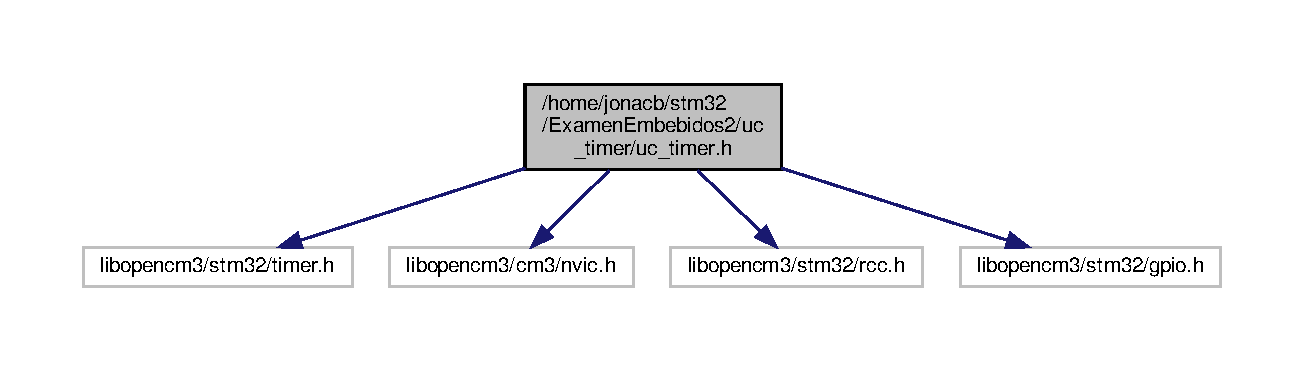
\includegraphics[width=350pt]{uc__timer_8h__incl}
\end{center}
\end{figure}
This graph shows which files directly or indirectly include this file\+:\nopagebreak
\begin{figure}[H]
\begin{center}
\leavevmode
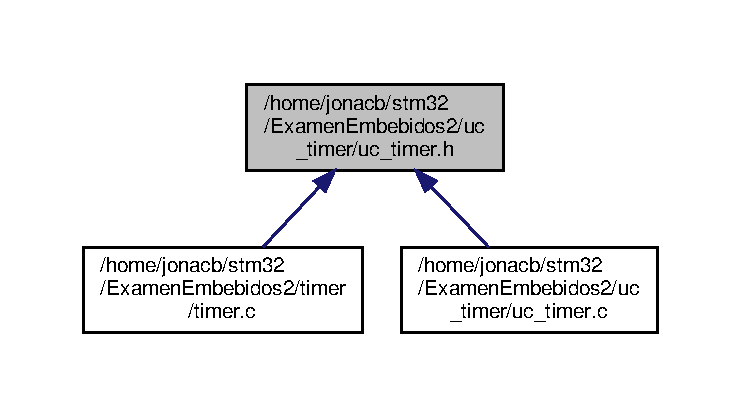
\includegraphics[width=350pt]{uc__timer_8h__dep__incl}
\end{center}
\end{figure}
\subsection*{Functions}
\begin{DoxyCompactItemize}
\item 
void \hyperlink{uc__timer_8h_a58293981ed0469d0d2b0cc0e70beecce}{uc\+\_\+timer\+\_\+pwm\+\_\+pin\+\_\+setup} (enum rcc\+\_\+periph\+\_\+clken gpio\+\_\+clk, uint32\+\_\+t gpio\+\_\+port, uint16\+\_\+t gpio\+\_\+pin)
\begin{DoxyCompactList}\small\item\em Sets up the P\+WM peripheral pin ports needed. \end{DoxyCompactList}\item 
void \hyperlink{uc__timer_8h_aa32fe1c6f887bf184010424db5634198}{uc\+\_\+timer\+\_\+setup} (enum rcc\+\_\+periph\+\_\+clken timer\+\_\+clk, uint32\+\_\+t timer, uint32\+\_\+t prescaler)
\begin{DoxyCompactList}\small\item\em Sets up the timer prescaler and enabled the clock. \end{DoxyCompactList}\item 
void \hyperlink{uc__timer_8h_a3783dcda7914f2a5113a276bbb6d886d}{uc\+\_\+timer\+\_\+pwm\+\_\+setup} (enum rcc\+\_\+periph\+\_\+clken timer\+\_\+clk, uint32\+\_\+t timer, enum tim\+\_\+oc\+\_\+id channel, uint32\+\_\+t prescaler)
\begin{DoxyCompactList}\small\item\em Enables and sets up the timer\textquotesingle{}s pwm. \end{DoxyCompactList}\item 
void \hyperlink{uc__timer_8h_a5ace3c51af58c627a2448d7af70f170f}{uc\+\_\+timer\+\_\+config\+\_\+period} (uint32\+\_\+t timer, uint32\+\_\+t period)
\begin{DoxyCompactList}\small\item\em Configures the timer\textquotesingle{}s period. \end{DoxyCompactList}\item 
void \hyperlink{uc__timer_8h_a1ca803f1f79b91d0fa7622bf5161b94e}{uc\+\_\+timer\+\_\+pwm\+\_\+config\+\_\+duty\+\_\+cycle} (uint32\+\_\+t timer, enum tim\+\_\+oc\+\_\+id channel, uint32\+\_\+t duty\+\_\+cycle)
\begin{DoxyCompactList}\small\item\em Configures the timer\textquotesingle{}s pwm duty cycle. \end{DoxyCompactList}\item 
void \hyperlink{uc__timer_8h_ac1f3c225897cfdee7111bcf69ffd0222}{uc\+\_\+timer\+\_\+enable\+\_\+interrupt} (uint32\+\_\+t timer, uint8\+\_\+t irqn)
\begin{DoxyCompactList}\small\item\em Enables timer\textquotesingle{}s interrupt. \end{DoxyCompactList}\item 
void \hyperlink{uc__timer_8h_a4962fd7b57586816079db0aa487091d3}{uc\+\_\+timer\+\_\+start} (uint32\+\_\+t timer)
\begin{DoxyCompactList}\small\item\em Starts the timer. \end{DoxyCompactList}\item 
void \hyperlink{uc__timer_8h_ab7c0468c8d4fc8bf514ada5ee90671e5}{uc\+\_\+timer\+\_\+stop} (uint32\+\_\+t timer)
\begin{DoxyCompactList}\small\item\em Stops the timer. \end{DoxyCompactList}\end{DoxyCompactItemize}


\subsection{Detailed Description}
uc\+\_\+timer header file. 



\subsection{Function Documentation}
\mbox{\Hypertarget{uc__timer_8h_a5ace3c51af58c627a2448d7af70f170f}\label{uc__timer_8h_a5ace3c51af58c627a2448d7af70f170f}} 
\index{uc\+\_\+timer.\+h@{uc\+\_\+timer.\+h}!uc\+\_\+timer\+\_\+config\+\_\+period@{uc\+\_\+timer\+\_\+config\+\_\+period}}
\index{uc\+\_\+timer\+\_\+config\+\_\+period@{uc\+\_\+timer\+\_\+config\+\_\+period}!uc\+\_\+timer.\+h@{uc\+\_\+timer.\+h}}
\subsubsection{\texorpdfstring{uc\+\_\+timer\+\_\+config\+\_\+period()}{uc\_timer\_config\_period()}}
{\footnotesize\ttfamily void uc\+\_\+timer\+\_\+config\+\_\+period (\begin{DoxyParamCaption}\item[{uint32\+\_\+t}]{timer,  }\item[{uint32\+\_\+t}]{period }\end{DoxyParamCaption})}



Configures the timer\textquotesingle{}s period. 


\begin{DoxyParams}[1]{Parameters}
\mbox{\tt in}  & {\em timer} & \\
\hline
\mbox{\tt in}  & {\em period} & \\
\hline
\end{DoxyParams}
\mbox{\Hypertarget{uc__timer_8h_ac1f3c225897cfdee7111bcf69ffd0222}\label{uc__timer_8h_ac1f3c225897cfdee7111bcf69ffd0222}} 
\index{uc\+\_\+timer.\+h@{uc\+\_\+timer.\+h}!uc\+\_\+timer\+\_\+enable\+\_\+interrupt@{uc\+\_\+timer\+\_\+enable\+\_\+interrupt}}
\index{uc\+\_\+timer\+\_\+enable\+\_\+interrupt@{uc\+\_\+timer\+\_\+enable\+\_\+interrupt}!uc\+\_\+timer.\+h@{uc\+\_\+timer.\+h}}
\subsubsection{\texorpdfstring{uc\+\_\+timer\+\_\+enable\+\_\+interrupt()}{uc\_timer\_enable\_interrupt()}}
{\footnotesize\ttfamily void uc\+\_\+timer\+\_\+enable\+\_\+interrupt (\begin{DoxyParamCaption}\item[{uint32\+\_\+t}]{timer,  }\item[{uint8\+\_\+t}]{irqn }\end{DoxyParamCaption})}



Enables timer\textquotesingle{}s interrupt. 


\begin{DoxyParams}[1]{Parameters}
\mbox{\tt in}  & {\em timer} & Timer used. \\
\hline
\mbox{\tt in}  & {\em irqn} & Timer Interrupt Service Request to be enabled. \\
\hline
\end{DoxyParams}
\mbox{\Hypertarget{uc__timer_8h_a1ca803f1f79b91d0fa7622bf5161b94e}\label{uc__timer_8h_a1ca803f1f79b91d0fa7622bf5161b94e}} 
\index{uc\+\_\+timer.\+h@{uc\+\_\+timer.\+h}!uc\+\_\+timer\+\_\+pwm\+\_\+config\+\_\+duty\+\_\+cycle@{uc\+\_\+timer\+\_\+pwm\+\_\+config\+\_\+duty\+\_\+cycle}}
\index{uc\+\_\+timer\+\_\+pwm\+\_\+config\+\_\+duty\+\_\+cycle@{uc\+\_\+timer\+\_\+pwm\+\_\+config\+\_\+duty\+\_\+cycle}!uc\+\_\+timer.\+h@{uc\+\_\+timer.\+h}}
\subsubsection{\texorpdfstring{uc\+\_\+timer\+\_\+pwm\+\_\+config\+\_\+duty\+\_\+cycle()}{uc\_timer\_pwm\_config\_duty\_cycle()}}
{\footnotesize\ttfamily void uc\+\_\+timer\+\_\+pwm\+\_\+config\+\_\+duty\+\_\+cycle (\begin{DoxyParamCaption}\item[{uint32\+\_\+t}]{timer,  }\item[{enum tim\+\_\+oc\+\_\+id}]{channel,  }\item[{uint32\+\_\+t}]{duty\+\_\+cycle }\end{DoxyParamCaption})}



Configures the timer\textquotesingle{}s pwm duty cycle. 


\begin{DoxyParams}[1]{Parameters}
\mbox{\tt in}  & {\em timer} & Timer used. \\
\hline
\mbox{\tt in}  & {\em channel} & Timer channel. \\
\hline
\mbox{\tt in}  & {\em duty\+\_\+cycle} & States the duty cycle of the timer. \\
\hline
\end{DoxyParams}
\mbox{\Hypertarget{uc__timer_8h_a58293981ed0469d0d2b0cc0e70beecce}\label{uc__timer_8h_a58293981ed0469d0d2b0cc0e70beecce}} 
\index{uc\+\_\+timer.\+h@{uc\+\_\+timer.\+h}!uc\+\_\+timer\+\_\+pwm\+\_\+pin\+\_\+setup@{uc\+\_\+timer\+\_\+pwm\+\_\+pin\+\_\+setup}}
\index{uc\+\_\+timer\+\_\+pwm\+\_\+pin\+\_\+setup@{uc\+\_\+timer\+\_\+pwm\+\_\+pin\+\_\+setup}!uc\+\_\+timer.\+h@{uc\+\_\+timer.\+h}}
\subsubsection{\texorpdfstring{uc\+\_\+timer\+\_\+pwm\+\_\+pin\+\_\+setup()}{uc\_timer\_pwm\_pin\_setup()}}
{\footnotesize\ttfamily void uc\+\_\+timer\+\_\+pwm\+\_\+pin\+\_\+setup (\begin{DoxyParamCaption}\item[{enum rcc\+\_\+periph\+\_\+clken}]{gpio\+\_\+clk,  }\item[{uint32\+\_\+t}]{gpio\+\_\+port,  }\item[{uint16\+\_\+t}]{gpio\+\_\+pin }\end{DoxyParamCaption})}



Sets up the P\+WM peripheral pin ports needed. 


\begin{DoxyParams}[1]{Parameters}
\mbox{\tt in}  & {\em gpio\+\_\+clk} & \\
\hline
\mbox{\tt in}  & {\em gpio\+\_\+port} & \\
\hline
\mbox{\tt in}  & {\em gpio\+\_\+pin} & \\
\hline
\end{DoxyParams}
\mbox{\Hypertarget{uc__timer_8h_a3783dcda7914f2a5113a276bbb6d886d}\label{uc__timer_8h_a3783dcda7914f2a5113a276bbb6d886d}} 
\index{uc\+\_\+timer.\+h@{uc\+\_\+timer.\+h}!uc\+\_\+timer\+\_\+pwm\+\_\+setup@{uc\+\_\+timer\+\_\+pwm\+\_\+setup}}
\index{uc\+\_\+timer\+\_\+pwm\+\_\+setup@{uc\+\_\+timer\+\_\+pwm\+\_\+setup}!uc\+\_\+timer.\+h@{uc\+\_\+timer.\+h}}
\subsubsection{\texorpdfstring{uc\+\_\+timer\+\_\+pwm\+\_\+setup()}{uc\_timer\_pwm\_setup()}}
{\footnotesize\ttfamily void uc\+\_\+timer\+\_\+pwm\+\_\+setup (\begin{DoxyParamCaption}\item[{enum rcc\+\_\+periph\+\_\+clken}]{timer\+\_\+clk,  }\item[{uint32\+\_\+t}]{timer,  }\item[{enum tim\+\_\+oc\+\_\+id}]{channel,  }\item[{uint32\+\_\+t}]{prescaler }\end{DoxyParamCaption})}



Enables and sets up the timer\textquotesingle{}s pwm. 


\begin{DoxyParams}[1]{Parameters}
\mbox{\tt in}  & {\em timer\+\_\+clk} & \\
\hline
\mbox{\tt in}  & {\em timer} & \\
\hline
\mbox{\tt in}  & {\em channel} & \\
\hline
\mbox{\tt in}  & {\em prescaler} & \\
\hline
\end{DoxyParams}
\mbox{\Hypertarget{uc__timer_8h_aa32fe1c6f887bf184010424db5634198}\label{uc__timer_8h_aa32fe1c6f887bf184010424db5634198}} 
\index{uc\+\_\+timer.\+h@{uc\+\_\+timer.\+h}!uc\+\_\+timer\+\_\+setup@{uc\+\_\+timer\+\_\+setup}}
\index{uc\+\_\+timer\+\_\+setup@{uc\+\_\+timer\+\_\+setup}!uc\+\_\+timer.\+h@{uc\+\_\+timer.\+h}}
\subsubsection{\texorpdfstring{uc\+\_\+timer\+\_\+setup()}{uc\_timer\_setup()}}
{\footnotesize\ttfamily void uc\+\_\+timer\+\_\+setup (\begin{DoxyParamCaption}\item[{enum rcc\+\_\+periph\+\_\+clken}]{timer\+\_\+clk,  }\item[{uint32\+\_\+t}]{timer,  }\item[{uint32\+\_\+t}]{prescaler }\end{DoxyParamCaption})}



Sets up the timer prescaler and enabled the clock. 


\begin{DoxyParams}[1]{Parameters}
\mbox{\tt in}  & {\em timer\+\_\+clk} & \\
\hline
\mbox{\tt in}  & {\em timer} & \\
\hline
\mbox{\tt in}  & {\em prescaler} & \\
\hline
\end{DoxyParams}
\mbox{\Hypertarget{uc__timer_8h_a4962fd7b57586816079db0aa487091d3}\label{uc__timer_8h_a4962fd7b57586816079db0aa487091d3}} 
\index{uc\+\_\+timer.\+h@{uc\+\_\+timer.\+h}!uc\+\_\+timer\+\_\+start@{uc\+\_\+timer\+\_\+start}}
\index{uc\+\_\+timer\+\_\+start@{uc\+\_\+timer\+\_\+start}!uc\+\_\+timer.\+h@{uc\+\_\+timer.\+h}}
\subsubsection{\texorpdfstring{uc\+\_\+timer\+\_\+start()}{uc\_timer\_start()}}
{\footnotesize\ttfamily void uc\+\_\+timer\+\_\+start (\begin{DoxyParamCaption}\item[{uint32\+\_\+t}]{timer }\end{DoxyParamCaption})}



Starts the timer. 


\begin{DoxyParams}[1]{Parameters}
\mbox{\tt in}  & {\em timer} & Timer used. \\
\hline
\end{DoxyParams}
\mbox{\Hypertarget{uc__timer_8h_ab7c0468c8d4fc8bf514ada5ee90671e5}\label{uc__timer_8h_ab7c0468c8d4fc8bf514ada5ee90671e5}} 
\index{uc\+\_\+timer.\+h@{uc\+\_\+timer.\+h}!uc\+\_\+timer\+\_\+stop@{uc\+\_\+timer\+\_\+stop}}
\index{uc\+\_\+timer\+\_\+stop@{uc\+\_\+timer\+\_\+stop}!uc\+\_\+timer.\+h@{uc\+\_\+timer.\+h}}
\subsubsection{\texorpdfstring{uc\+\_\+timer\+\_\+stop()}{uc\_timer\_stop()}}
{\footnotesize\ttfamily void uc\+\_\+timer\+\_\+stop (\begin{DoxyParamCaption}\item[{uint32\+\_\+t}]{timer }\end{DoxyParamCaption})}



Stops the timer. 


\begin{DoxyParams}[1]{Parameters}
\mbox{\tt in}  & {\em timer} & Timer used. \\
\hline
\end{DoxyParams}

\hypertarget{uc__uart_8c}{}\section{/home/jonacb/stm32/\+Examen\+Embebidos2/uc\+\_\+uart/uc\+\_\+uart.c File Reference}
\label{uc__uart_8c}\index{/home/jonacb/stm32/\+Examen\+Embebidos2/uc\+\_\+uart/uc\+\_\+uart.\+c@{/home/jonacb/stm32/\+Examen\+Embebidos2/uc\+\_\+uart/uc\+\_\+uart.\+c}}


uc\+\_\+uart function definitions.  


{\ttfamily \#include \char`\"{}uc\+\_\+uart.\+h\char`\"{}}\newline
{\ttfamily \#include $<$libopencm3/stm32/usart.\+h$>$}\newline
{\ttfamily \#include $<$libopencm3/cm3/nvic.\+h$>$}\newline
{\ttfamily \#include $<$libopencm3/stm32/rcc.\+h$>$}\newline
{\ttfamily \#include $<$libopencm3/stm32/gpio.\+h$>$}\newline
{\ttfamily \#include \char`\"{}../miniprintf/miniprintf.\+h\char`\"{}}\newline
Include dependency graph for uc\+\_\+uart.\+c\+:\nopagebreak
\begin{figure}[H]
\begin{center}
\leavevmode
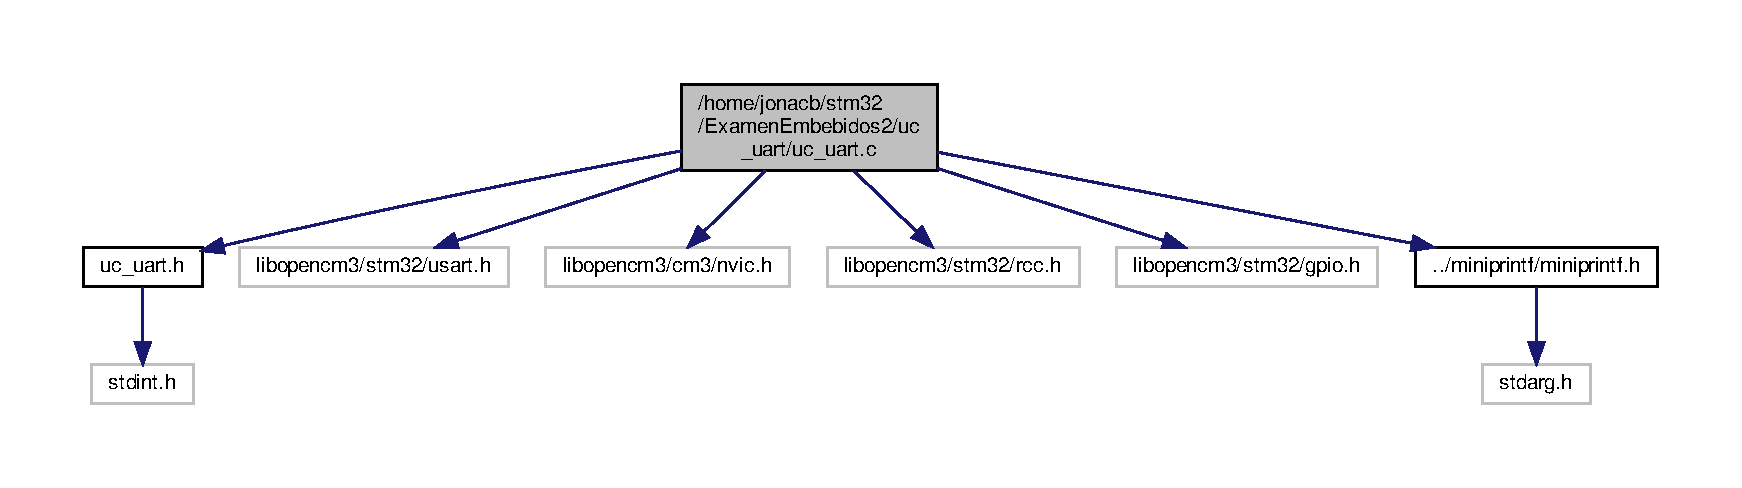
\includegraphics[width=350pt]{uc__uart_8c__incl}
\end{center}
\end{figure}
\subsection*{Functions}
\begin{DoxyCompactItemize}
\item 
void \hyperlink{uc__uart_8c_ae468e0937557eefb10705cec62e1599b}{uart\+\_\+putc} (char ch)
\begin{DoxyCompactList}\small\item\em Sends a char. \end{DoxyCompactList}\item 
int \hyperlink{uc__uart_8c_a953fcdef2bec3905b52c22983a8567eb}{uart\+\_\+printf} (const char $\ast$format,...)
\begin{DoxyCompactList}\small\item\em Prints U\+A\+RT message. \end{DoxyCompactList}\item 
void \hyperlink{uc__uart_8c_a4c32397c8b24d1f414bb4ace805c795e}{uart\+\_\+pin\+\_\+setup} (uint32\+\_\+t tx\+\_\+port, uint32\+\_\+t tx\+\_\+pin, uint32\+\_\+t rx\+\_\+port, uint32\+\_\+t rx\+\_\+pin)
\begin{DoxyCompactList}\small\item\em Sets up the U\+A\+RT peripheral pin ports needed. \end{DoxyCompactList}\item 
void \hyperlink{uc__uart_8c_a65773aa4e29491601b9ec336332fb8c4}{uart\+\_\+setup} (uint32\+\_\+t uart, uint32\+\_\+t baudrate, uint32\+\_\+t databits)
\begin{DoxyCompactList}\small\item\em Sets up the U\+A\+RT configuration. \end{DoxyCompactList}\item 
void \hyperlink{uc__uart_8c_a4b03985035c306b5819e23671abfe049}{uart\+\_\+start} (uint32\+\_\+t uart)
\begin{DoxyCompactList}\small\item\em Starts U\+A\+RT. \end{DoxyCompactList}\end{DoxyCompactItemize}
\subsection*{Variables}
\begin{DoxyCompactItemize}
\item 
uint32\+\_\+t \hyperlink{uc__uart_8c_a206ca77a1a1fcafd37f2e07532397bdc}{current\+\_\+uart}
\begin{DoxyCompactList}\small\item\em $<$Miniprint library include. \end{DoxyCompactList}\end{DoxyCompactItemize}


\subsection{Detailed Description}
uc\+\_\+uart function definitions. 



\subsection{Function Documentation}
\mbox{\Hypertarget{uc__uart_8c_a4c32397c8b24d1f414bb4ace805c795e}\label{uc__uart_8c_a4c32397c8b24d1f414bb4ace805c795e}} 
\index{uc\+\_\+uart.\+c@{uc\+\_\+uart.\+c}!uart\+\_\+pin\+\_\+setup@{uart\+\_\+pin\+\_\+setup}}
\index{uart\+\_\+pin\+\_\+setup@{uart\+\_\+pin\+\_\+setup}!uc\+\_\+uart.\+c@{uc\+\_\+uart.\+c}}
\subsubsection{\texorpdfstring{uart\+\_\+pin\+\_\+setup()}{uart\_pin\_setup()}}
{\footnotesize\ttfamily void uart\+\_\+pin\+\_\+setup (\begin{DoxyParamCaption}\item[{uint32\+\_\+t}]{tx\+\_\+port,  }\item[{uint32\+\_\+t}]{tx\+\_\+pin,  }\item[{uint32\+\_\+t}]{rx\+\_\+port,  }\item[{uint32\+\_\+t}]{rx\+\_\+pin }\end{DoxyParamCaption})}



Sets up the U\+A\+RT peripheral pin ports needed. 


\begin{DoxyParams}[1]{Parameters}
\mbox{\tt in}  & {\em tx\+\_\+port} & Specifies the port of the U\+A\+RT transmitter. \\
\hline
\mbox{\tt in}  & {\em tx\+\_\+pin} & Specifies the pin of the U\+A\+RT transmitter. \\
\hline
\mbox{\tt in}  & {\em rx\+\_\+port} & Specifies the port of the U\+A\+RT receiver. \\
\hline
\mbox{\tt in}  & {\em rx\+\_\+pin} & Specifies the pin of the U\+A\+RT receiver. \\
\hline
\end{DoxyParams}
\mbox{\Hypertarget{uc__uart_8c_a953fcdef2bec3905b52c22983a8567eb}\label{uc__uart_8c_a953fcdef2bec3905b52c22983a8567eb}} 
\index{uc\+\_\+uart.\+c@{uc\+\_\+uart.\+c}!uart\+\_\+printf@{uart\+\_\+printf}}
\index{uart\+\_\+printf@{uart\+\_\+printf}!uc\+\_\+uart.\+c@{uc\+\_\+uart.\+c}}
\subsubsection{\texorpdfstring{uart\+\_\+printf()}{uart\_printf()}}
{\footnotesize\ttfamily int uart\+\_\+printf (\begin{DoxyParamCaption}\item[{const char $\ast$}]{format,  }\item[{}]{... }\end{DoxyParamCaption})}



Prints U\+A\+RT message. 


\begin{DoxyParams}[1]{Parameters}
\mbox{\tt in}  & {\em format} & String format. \\
\hline
\end{DoxyParams}
\begin{DoxyReturn}{Returns}
rc 
\end{DoxyReturn}
\mbox{\Hypertarget{uc__uart_8c_ae468e0937557eefb10705cec62e1599b}\label{uc__uart_8c_ae468e0937557eefb10705cec62e1599b}} 
\index{uc\+\_\+uart.\+c@{uc\+\_\+uart.\+c}!uart\+\_\+putc@{uart\+\_\+putc}}
\index{uart\+\_\+putc@{uart\+\_\+putc}!uc\+\_\+uart.\+c@{uc\+\_\+uart.\+c}}
\subsubsection{\texorpdfstring{uart\+\_\+putc()}{uart\_putc()}}
{\footnotesize\ttfamily void uart\+\_\+putc (\begin{DoxyParamCaption}\item[{char}]{ch }\end{DoxyParamCaption})}



Sends a char. 


\begin{DoxyParams}[1]{Parameters}
\mbox{\tt in}  & {\em ch} & Char to be transmitted. \\
\hline
\end{DoxyParams}
\mbox{\Hypertarget{uc__uart_8c_a65773aa4e29491601b9ec336332fb8c4}\label{uc__uart_8c_a65773aa4e29491601b9ec336332fb8c4}} 
\index{uc\+\_\+uart.\+c@{uc\+\_\+uart.\+c}!uart\+\_\+setup@{uart\+\_\+setup}}
\index{uart\+\_\+setup@{uart\+\_\+setup}!uc\+\_\+uart.\+c@{uc\+\_\+uart.\+c}}
\subsubsection{\texorpdfstring{uart\+\_\+setup()}{uart\_setup()}}
{\footnotesize\ttfamily void uart\+\_\+setup (\begin{DoxyParamCaption}\item[{uint32\+\_\+t}]{uart,  }\item[{uint32\+\_\+t}]{baudrate,  }\item[{uint32\+\_\+t}]{databits }\end{DoxyParamCaption})}



Sets up the U\+A\+RT configuration. 


\begin{DoxyParams}[1]{Parameters}
\mbox{\tt in}  & {\em uart} & U\+A\+RT to be used. \\
\hline
\mbox{\tt in}  & {\em baudrate} & Baudrate used for U\+A\+RT communication. \\
\hline
\mbox{\tt in}  & {\em databits} & Message data width. \\
\hline
\end{DoxyParams}
\mbox{\Hypertarget{uc__uart_8c_a4b03985035c306b5819e23671abfe049}\label{uc__uart_8c_a4b03985035c306b5819e23671abfe049}} 
\index{uc\+\_\+uart.\+c@{uc\+\_\+uart.\+c}!uart\+\_\+start@{uart\+\_\+start}}
\index{uart\+\_\+start@{uart\+\_\+start}!uc\+\_\+uart.\+c@{uc\+\_\+uart.\+c}}
\subsubsection{\texorpdfstring{uart\+\_\+start()}{uart\_start()}}
{\footnotesize\ttfamily void uart\+\_\+start (\begin{DoxyParamCaption}\item[{uint32\+\_\+t}]{uart }\end{DoxyParamCaption})}



Starts U\+A\+RT. 


\begin{DoxyParams}[1]{Parameters}
\mbox{\tt in}  & {\em uart} & U\+A\+RT to be used. \\
\hline
\end{DoxyParams}


\subsection{Variable Documentation}
\mbox{\Hypertarget{uc__uart_8c_a206ca77a1a1fcafd37f2e07532397bdc}\label{uc__uart_8c_a206ca77a1a1fcafd37f2e07532397bdc}} 
\index{uc\+\_\+uart.\+c@{uc\+\_\+uart.\+c}!current\+\_\+uart@{current\+\_\+uart}}
\index{current\+\_\+uart@{current\+\_\+uart}!uc\+\_\+uart.\+c@{uc\+\_\+uart.\+c}}
\subsubsection{\texorpdfstring{current\+\_\+uart}{current\_uart}}
{\footnotesize\ttfamily uint32\+\_\+t current\+\_\+uart}



$<$Miniprint library include. 

$<$U\+A\+RT custom defines. $<$libopencm3 U\+S\+A\+RT functions. $<$libopencm3 N\+V\+IC functions. $<$libopencm3 R\+CC functions. $<$libopencm3 G\+P\+IO functions.\+Currently used U\+A\+RT. 
\hypertarget{uc__uart_8h}{}\section{/home/jonacb/stm32/\+Examen\+Embebidos2/uc\+\_\+uart/uc\+\_\+uart.h File Reference}
\label{uc__uart_8h}\index{/home/jonacb/stm32/\+Examen\+Embebidos2/uc\+\_\+uart/uc\+\_\+uart.\+h@{/home/jonacb/stm32/\+Examen\+Embebidos2/uc\+\_\+uart/uc\+\_\+uart.\+h}}


U\+A\+RT I\+N\+C\+L\+U\+D\+ES.  


{\ttfamily \#include $<$stdint.\+h$>$}\newline
Include dependency graph for uc\+\_\+uart.\+h\+:\nopagebreak
\begin{figure}[H]
\begin{center}
\leavevmode
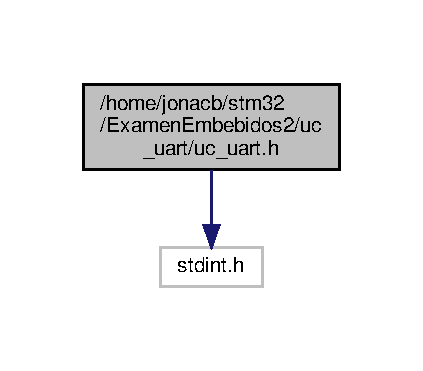
\includegraphics[width=203pt]{uc__uart_8h__incl}
\end{center}
\end{figure}
This graph shows which files directly or indirectly include this file\+:\nopagebreak
\begin{figure}[H]
\begin{center}
\leavevmode
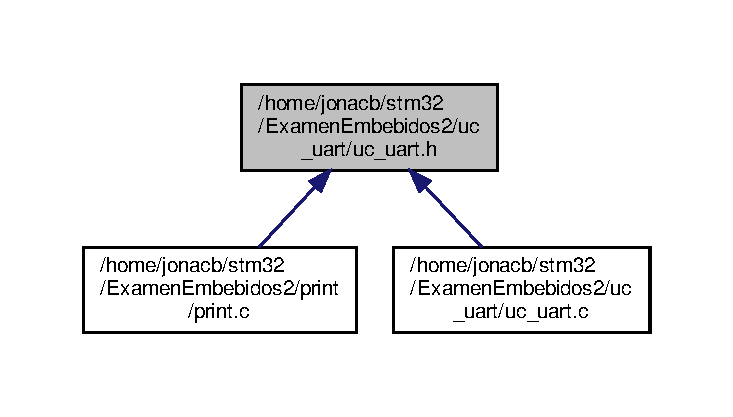
\includegraphics[width=350pt]{uc__uart_8h__dep__incl}
\end{center}
\end{figure}
\subsection*{Functions}
\begin{DoxyCompactItemize}
\item 
void \hyperlink{uc__uart_8h_a4c32397c8b24d1f414bb4ace805c795e}{uart\+\_\+pin\+\_\+setup} (uint32\+\_\+t tx\+\_\+port, uint32\+\_\+t tx\+\_\+pin, uint32\+\_\+t rx\+\_\+port, uint32\+\_\+t rx\+\_\+pin)
\begin{DoxyCompactList}\small\item\em Sets up the U\+A\+RT peripheral pin ports needed. \end{DoxyCompactList}\item 
void \hyperlink{uc__uart_8h_a65773aa4e29491601b9ec336332fb8c4}{uart\+\_\+setup} (uint32\+\_\+t uart, uint32\+\_\+t baudrate, uint32\+\_\+t databits)
\begin{DoxyCompactList}\small\item\em Sets up the U\+A\+RT configuration. \end{DoxyCompactList}\item 
void \hyperlink{uc__uart_8h_a4b03985035c306b5819e23671abfe049}{uart\+\_\+start} (uint32\+\_\+t uart)
\begin{DoxyCompactList}\small\item\em Starts U\+A\+RT. \end{DoxyCompactList}\item 
void \hyperlink{uc__uart_8h_ae468e0937557eefb10705cec62e1599b}{uart\+\_\+putc} (char ch)
\begin{DoxyCompactList}\small\item\em Sends a char. \end{DoxyCompactList}\item 
int \hyperlink{uc__uart_8h_a953fcdef2bec3905b52c22983a8567eb}{uart\+\_\+printf} (const char $\ast$format,...)
\begin{DoxyCompactList}\small\item\em Prints U\+A\+RT message. \end{DoxyCompactList}\end{DoxyCompactItemize}


\subsection{Detailed Description}
U\+A\+RT I\+N\+C\+L\+U\+D\+ES. 



\subsection{Function Documentation}
\mbox{\Hypertarget{uc__uart_8h_a4c32397c8b24d1f414bb4ace805c795e}\label{uc__uart_8h_a4c32397c8b24d1f414bb4ace805c795e}} 
\index{uc\+\_\+uart.\+h@{uc\+\_\+uart.\+h}!uart\+\_\+pin\+\_\+setup@{uart\+\_\+pin\+\_\+setup}}
\index{uart\+\_\+pin\+\_\+setup@{uart\+\_\+pin\+\_\+setup}!uc\+\_\+uart.\+h@{uc\+\_\+uart.\+h}}
\subsubsection{\texorpdfstring{uart\+\_\+pin\+\_\+setup()}{uart\_pin\_setup()}}
{\footnotesize\ttfamily void uart\+\_\+pin\+\_\+setup (\begin{DoxyParamCaption}\item[{uint32\+\_\+t}]{tx\+\_\+port,  }\item[{uint32\+\_\+t}]{tx\+\_\+pin,  }\item[{uint32\+\_\+t}]{rx\+\_\+port,  }\item[{uint32\+\_\+t}]{rx\+\_\+pin }\end{DoxyParamCaption})}



Sets up the U\+A\+RT peripheral pin ports needed. 


\begin{DoxyParams}[1]{Parameters}
\mbox{\tt in}  & {\em tx\+\_\+port} & Specifies the port of the U\+A\+RT transmitter. \\
\hline
\mbox{\tt in}  & {\em tx\+\_\+pin} & Specifies the pin of the U\+A\+RT transmitter. \\
\hline
\mbox{\tt in}  & {\em rx\+\_\+port} & Specifies the port of the U\+A\+RT receiver. \\
\hline
\mbox{\tt in}  & {\em rx\+\_\+pin} & Specifies the pin of the U\+A\+RT receiver. \\
\hline
\end{DoxyParams}
\mbox{\Hypertarget{uc__uart_8h_a953fcdef2bec3905b52c22983a8567eb}\label{uc__uart_8h_a953fcdef2bec3905b52c22983a8567eb}} 
\index{uc\+\_\+uart.\+h@{uc\+\_\+uart.\+h}!uart\+\_\+printf@{uart\+\_\+printf}}
\index{uart\+\_\+printf@{uart\+\_\+printf}!uc\+\_\+uart.\+h@{uc\+\_\+uart.\+h}}
\subsubsection{\texorpdfstring{uart\+\_\+printf()}{uart\_printf()}}
{\footnotesize\ttfamily int uart\+\_\+printf (\begin{DoxyParamCaption}\item[{const char $\ast$}]{format,  }\item[{}]{... }\end{DoxyParamCaption})}



Prints U\+A\+RT message. 


\begin{DoxyParams}[1]{Parameters}
\mbox{\tt in}  & {\em format} & String format. \\
\hline
\end{DoxyParams}
\begin{DoxyReturn}{Returns}
rc 
\end{DoxyReturn}
\mbox{\Hypertarget{uc__uart_8h_ae468e0937557eefb10705cec62e1599b}\label{uc__uart_8h_ae468e0937557eefb10705cec62e1599b}} 
\index{uc\+\_\+uart.\+h@{uc\+\_\+uart.\+h}!uart\+\_\+putc@{uart\+\_\+putc}}
\index{uart\+\_\+putc@{uart\+\_\+putc}!uc\+\_\+uart.\+h@{uc\+\_\+uart.\+h}}
\subsubsection{\texorpdfstring{uart\+\_\+putc()}{uart\_putc()}}
{\footnotesize\ttfamily void uart\+\_\+putc (\begin{DoxyParamCaption}\item[{char}]{ch }\end{DoxyParamCaption})}



Sends a char. 


\begin{DoxyParams}[1]{Parameters}
\mbox{\tt in}  & {\em ch} & Char to be transmitted. \\
\hline
\end{DoxyParams}
\mbox{\Hypertarget{uc__uart_8h_a65773aa4e29491601b9ec336332fb8c4}\label{uc__uart_8h_a65773aa4e29491601b9ec336332fb8c4}} 
\index{uc\+\_\+uart.\+h@{uc\+\_\+uart.\+h}!uart\+\_\+setup@{uart\+\_\+setup}}
\index{uart\+\_\+setup@{uart\+\_\+setup}!uc\+\_\+uart.\+h@{uc\+\_\+uart.\+h}}
\subsubsection{\texorpdfstring{uart\+\_\+setup()}{uart\_setup()}}
{\footnotesize\ttfamily void uart\+\_\+setup (\begin{DoxyParamCaption}\item[{uint32\+\_\+t}]{uart,  }\item[{uint32\+\_\+t}]{baudrate,  }\item[{uint32\+\_\+t}]{databits }\end{DoxyParamCaption})}



Sets up the U\+A\+RT configuration. 


\begin{DoxyParams}[1]{Parameters}
\mbox{\tt in}  & {\em uart} & U\+A\+RT to be used. \\
\hline
\mbox{\tt in}  & {\em baudrate} & Baudrate used for U\+A\+RT communication. \\
\hline
\mbox{\tt in}  & {\em databits} & Message data width. \\
\hline
\end{DoxyParams}
\mbox{\Hypertarget{uc__uart_8h_a4b03985035c306b5819e23671abfe049}\label{uc__uart_8h_a4b03985035c306b5819e23671abfe049}} 
\index{uc\+\_\+uart.\+h@{uc\+\_\+uart.\+h}!uart\+\_\+start@{uart\+\_\+start}}
\index{uart\+\_\+start@{uart\+\_\+start}!uc\+\_\+uart.\+h@{uc\+\_\+uart.\+h}}
\subsubsection{\texorpdfstring{uart\+\_\+start()}{uart\_start()}}
{\footnotesize\ttfamily void uart\+\_\+start (\begin{DoxyParamCaption}\item[{uint32\+\_\+t}]{uart }\end{DoxyParamCaption})}



Starts U\+A\+RT. 


\begin{DoxyParams}[1]{Parameters}
\mbox{\tt in}  & {\em uart} & U\+A\+RT to be used. \\
\hline
\end{DoxyParams}

%--- End generated contents ---

% Index
\backmatter
\newpage
\phantomsection
\clearemptydoublepage
\addcontentsline{toc}{chapter}{Index}
\printindex

\end{document}
